%% Springer Nature LaTeX template — sn-jnl class (December 2024)
%% Compile with: pdflatex -> bibtex -> pdflatex -> pdflatex

\documentclass[pdflatex,sn-basic]{sn-jnl}

%%%% Standard packages
\usepackage{amsmath,amssymb,amsfonts}
\usepackage{graphicx}
\usepackage{xcolor}
\usepackage{float}
\usepackage{booktabs}
\usepackage{multirow}
\usepackage{makecell}
\usepackage{url}
\usepackage{hyperref}
\usepackage{tikz}
\usetikzlibrary{
    arrows.meta,
    shapes.geometric,
    shapes,
    arrows,
    positioning,
    fit,
    backgrounds,
    calc,
    matrix,
    decorations.pathreplacing
}


\begin{document}

\title[Hybrid CNN Feature Stacking for Crop Health Assessment]
      {A Robust and Interpretable Deep Learning Framework for Crop Health Assessment Using Hybrid CNN Feature Stacking}

\author*[1]{\fnm{Pape ElHadji Abdoulaye} \sur{Gueye}}\email{papeabdoulaye.gueye@uadb.edu.sn}
\equalcont{Corresponding author.}

\author[1]{\fnm{Cherif Bachir} \sur{Deme}}
\author[1]{\fnm{Diery} \sur{Ngom}}
\author[1]{\fnm{Adrien} \sur{Basse}}

\affil*[1]{\orgdiv{Department of ICT, UFR SATIC},
           \orgname{Alioune Diop University},
           \orgaddress{\street{BP 30}, \city{Bambey}, \country{Senegal}}}

\abstract{

Ensuring food security in climate-vulnerable regions such as Senegal requires timely crop health monitoring. While deep learning has advanced plant disease detection, single-model approaches often lack generalizability and interpretability. We present a hybrid feature-level stacking framework combining three pre-trained CNNs—ResNet50, EfficientNetB0, and MobileNetV2—to enhance classification robustness. Extracted features are processed by three meta-learners: a full MLP, an MLP with PCA preprocessing, and a harmonized PCA-Logistic pipeline on 790 components.

Evaluated on the PlantVillage dataset (54,306 images, 38 classes), the full MLP achieves \textbf{95.82\% test accuracy}, outperforming individual backbones by 1.9--2.7 points. Statistical analysis shows 95\% of feature variance is captured by 790 components, yielding a \textbf{5.8$\times$ compression ratio}. Low inter-backbone correlation (0.086) confirms complementarity: ResNet50 captures deep semantic features (MI\,=\,0.152), EfficientNetB0 provides multi-scale representations (MI\,=\,0.138), and MobileNetV2 encodes texture patterns (MI\,=\,0.131). The PCA-Logistic variant reaches \textbf{94.61\% accuracy} (98.7\% of full MLP) with a \textbf{6.3$\times$ training speedup}, while MLP-PCA retains \textbf{94.86\% accuracy} using only 17.1\% of features. McNemar's tests show MLP-Full significantly outperforms PCA-based models ($p < 10^{-6}$), with no significant difference between MLP-PCA and PCA-Logistic ($p = 0.253$). SHAP explainability confirms that all backbones contribute meaningfully, with feature importance aligned with mutual information scores and decisions focused on biologically relevant disease regions.

This framework overcomes limitations of single-model CNNs via multi-backbone fusion, integrated interpretability, and flexible accuracy-efficiency trade-offs, providing a practical AI-assisted solution for crop monitoring in resource-constrained environments.

}

\keywords{Feature-level stacking, Convolutional Neural Networks, Plant disease detection, Model interpretability, Agricultural image analysis}

\maketitle

%%--------------------------------------------------------------------
\section{Introduction}
\label{sec:intro}
%%--------------------------------------------------------------------

Monitoring crop health accurately and at scale remains one of the most pressing challenges in modern agriculture, particularly in regions exposed to high climatic variability such as Senegal. The country faces irregular rainfall, recurring droughts, and rising temperatures, all of which place increasing pressure on agricultural productivity and food security~\cite{koseki_dakar_2024}. Traditional approaches based on visual field inspection and expert judgment are time-consuming, difficult to scale, and inherently subjective. They fall short of capturing the complex and dynamic interactions among climatic, environmental, and agronomic factors that characterize real agricultural settings~\cite{misbah_multi-sensors_2021}.

Against this backdrop, deep learning and Convolutional Neural Networks (CNNs) in particular have emerged as a powerful paradigm for plant disease detection and crop monitoring from image data. A recent study by Hussain et al.~\cite{mir_deep_2025} demonstrated how deep learning can strengthen IoT-based crop monitoring by automating greenhouse surveillance and environmental regulation. Their framework couples sensor data with advanced activation functions (ELU, Swish, ReLU, SELU, and Mish) to reduce human intervention and improve sustainability. While the results are encouraging, the approach is confined to controlled greenhouse conditions and does not readily extend to open-field scenarios.

Several comparative studies have further benchmarked popular CNN architectures for crop health monitoring. Suresh Manic et al.~\cite{SureshManic2025} evaluated EfficientNetB0, InceptionV3, DenseNet121, and MobileNetV2, finding that EfficientNetB0 achieved the highest validation accuracy (96.4\%) while remaining suitable for edge deployment in resource-constrained environments. González-Briones et al.~\cite{GonzalezBriones2025} showed that ResNet-50 and EfficientNet, when paired with explainability mechanisms, achieve respectively 63.79\% and 98.27\% accuracy on PlantVillage, underscoring that architecture choice involves trade-offs among accuracy, robustness, and interpretability. These findings point to a broader consensus: no single architecture dominates across all conditions, and transparency is increasingly recognized as a deployment requirement rather than an optional feature.

Beyond ground-level imaging, UAV-based remote sensing has also been explored for large-scale crop monitoring. Zhang et al.~\cite{Zhang2024} investigated how deep learning can be applied to aerial imagery from unmanned vehicles to detect diseases and pests across wide agricultural areas. Although promising in scope, this line of work still faces challenges related to data variability, model generalization, and the computational demands of real-time processing at scale.

Islam et al.~\cite{Islam2023} proposed DeepCrop, a deep learning framework for crop disease prediction that compared CNN, VGG-16, VGG-19, and ResNet-50 on the PlantVillage dataset. ResNet-50 emerged as the best-performing architecture with 98.98\% accuracy and robust cross-validation results. Beyond model performance, the authors developed a web application that allows farmers to upload leaf images for real-time diagnosis and treatment suggestions, demonstrating how research-grade models can be embedded into accessible tools for smallholder farmers. Their study nonetheless remains limited to controlled benchmark data and does not address the challenge of field-collected images.

Yakkala et al.~\cite{Yakkala2024} developed an early disease prediction framework based on ResNet-9, which classifies healthy and diseased leaves from morphological features including color, intensity, and spatial dimensions. The model showed high accuracy supported by systematic preprocessing and augmentation strategies, and the authors made a point of integrating their approach with biological control methods, positioning it as both technologically sound and ecologically responsible.

Despite these advances, most existing methods share a common structural limitation: they rely on a single model architecture, whether ResNet50, EfficientNet, or MobileNetV2, which inevitably captures only a partial view of the visual information present in plant disease images. Models trained on controlled benchmark datasets like PlantVillage frequently suffer from domain shift when applied to real agricultural conditions, including images captured in the field, by drones, or under variable illumination. This leads to overfitting and reduced robustness in practical deployment. Furthermore, most studies focus exclusively on end-to-end classification without exploiting the complementary strengths of multiple architectures or providing meaningful insight into how predictions are made. The result is systems that may perform well on benchmarks but remain opaque and fragile in practice.

To address these challenges, we propose a \textbf{hybrid feature-level stacking framework} that fuses deep representations from three complementary CNN architectures: \textbf{ResNet50}, \textbf{EfficientNetB0}, and \textbf{MobileNetV2}. Rather than aggregating final predictions, our approach extracts and concatenates intermediate feature vectors, which are then processed by a meta-learner for classification. We systematically evaluate three meta-learner variants: a full MLP, an MLP with PCA preprocessing, and a harmonized PCA-Logistic pipeline using 790 components. The framework incorporates comprehensive statistical analysis, regularization, cross-validation, and paired statistical tests. Transparency is ensured through SHAP-based global feature importance analysis.

The main contributions of this work are fourfold:
\begin{enumerate}
    \item A \textbf{multi-backbone feature fusion} strategy that leverages complementary representations from ResNet50 (deep semantic features), EfficientNetB0 (multi-scale representations), and MobileNetV2 (lightweight texture patterns), achieving \textbf{95.82\% test accuracy} and outperforming any single backbone by 1.9 to 2.7 percentage points.

    \item \textbf{Comprehensive statistical analysis} revealing substantial feature redundancy ($5.8\times$ compression at 95\% variance retention) alongside low inter-backbone correlation (0.086), which confirms architectural complementarity with mean Mutual Information scores of 0.152 (ResNet50), 0.138 (EfficientNetB0), and 0.131 (MobileNetV2).

    \item \textbf{Systematic evaluation of meta-learners} exposing meaningful accuracy-efficiency trade-offs: MLP-Full (\textbf{95.82\% accuracy}), harmonized PCA-Logistic (\textbf{94.61\% accuracy}, $6.3\times$ faster training), and MLP-PCA (\textbf{94.86\% accuracy} with only 17.1\% of original features). McNemar's tests confirm that MLP-Full significantly outperforms PCA-based models ($p < 10^{-6}$), with no significant difference between MLP-PCA and PCA-Logistic ($p = 0.253$).

    \item \textbf{Integrated explainability} confirming that all three backbones contribute meaningfully to classification, with models focusing on biologically relevant regions such as lesions, spots, and discolouration patterns rather than incidental background correlations.
\end{enumerate}

The proposed framework advances existing approaches on several fronts: it improves robustness through multi-model feature fusion, promotes transparency through integrated explainability, enables significant dimensionality reduction without performance loss, and offers deployment options suited to varying resource constraints. These properties are particularly relevant for agricultural monitoring in settings like Senegal, where climate variability threatens crop productivity and where reliable, interpretable AI tools are urgently needed.

The remainder of this paper is organized as follows. Section~\ref{sec:methodology} describes the methodology, covering data preprocessing, multi-backbone feature extraction, statistical feature analysis, meta-learner architectures, and validation strategies. Section~\ref{sec:results} presents experimental results, including feature statistics, model performance comparisons, statistical significance tests, and interpretability findings. Section~\ref{sec:discussion} discusses the implications of the results, limitations, and directions for future work. Section~\ref{sec:conclusion} concludes with key contributions and practical recommendations for deployment.

%%--------------------------------------------------------------------
\section{Methodology}
\label{sec:methodology}
%%--------------------------------------------------------------------

\subsection{Overall Architecture}
\label{subsec:architecture}

The proposed framework follows a two-stage hierarchical architecture(Figure~\ref{fig:architecture}) designed to extract and combine complementary visual representations from multiple pre-trained CNNs. In the first stage, three distinct backbone architectures independently transform input images into high-dimensional feature vectors. In the second stage, these vectors are fused and passed to one of three meta-learner variants: a full MLP operating on all extracted features, an MLP preceded by PCA dimensionality reduction, and a harmonized PCA-Logistic Regression pipeline using exactly 790 components. Evaluating all three variants in parallel allows us to rigorously characterize the trade-offs between representational capacity, computational efficiency, and statistical robustness, rather than committing to a single design choice.

\begin{figure}[htbp]
\centering
\resizebox{\textwidth}{!}{%
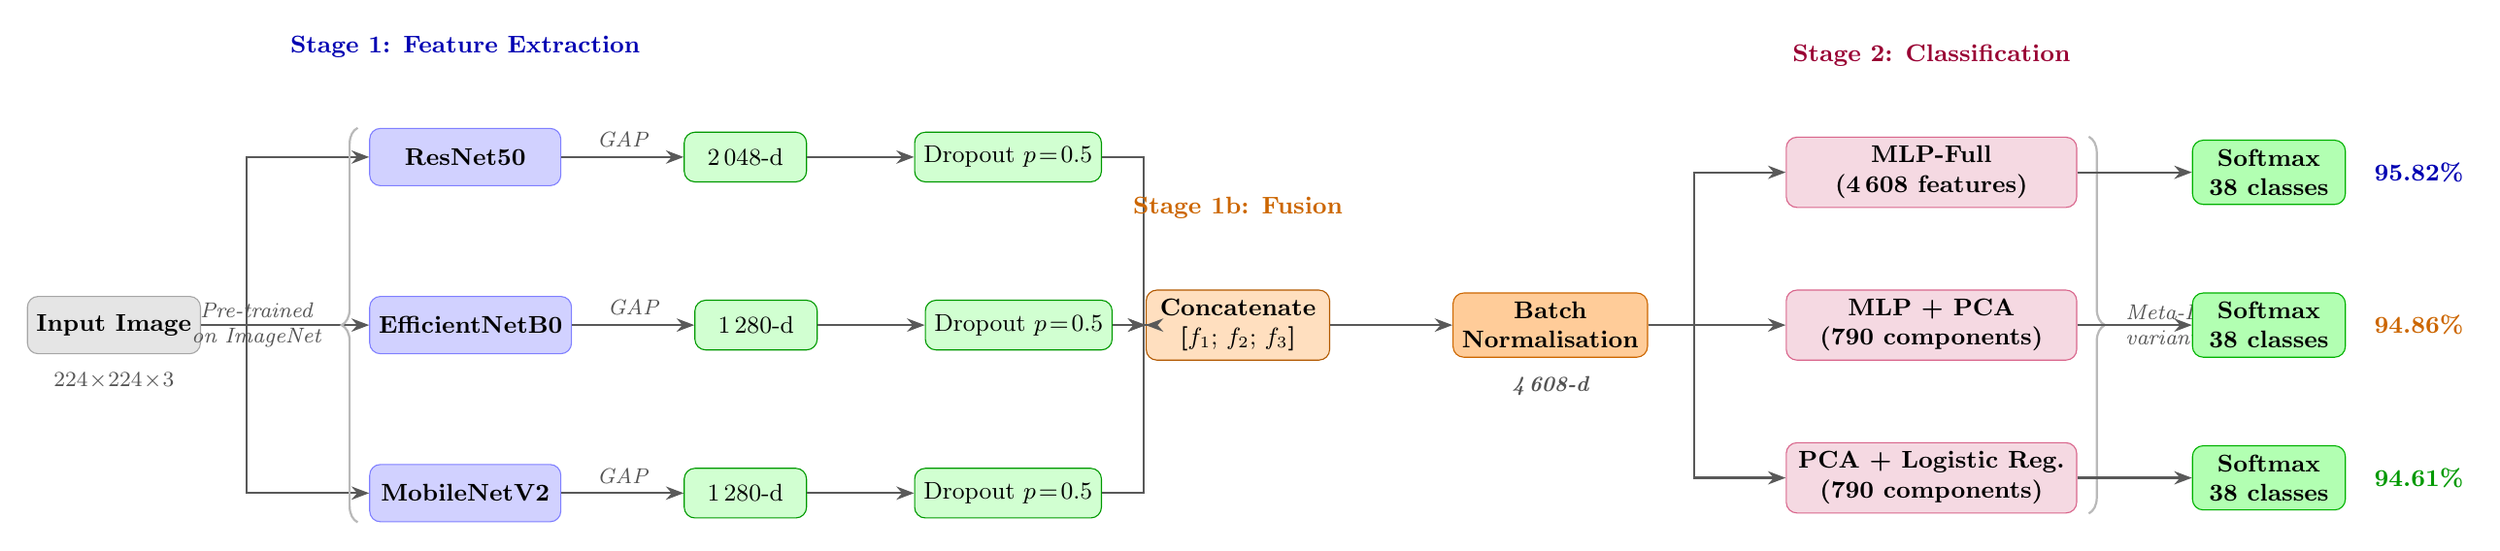
\begin{tikzpicture}[
  input/.style={rectangle, rounded corners=4pt,
    draw=gray!70, fill=gray!20,
    minimum width=2.2cm, minimum height=0.75cm,
    font=\small\bfseries, align=center},
  backbone/.style={rectangle, rounded corners=4pt,
    draw=blue!50, fill=blue!18,
    minimum width=2.5cm, minimum height=0.75cm,
    font=\small\bfseries, align=center},
  feat/.style={rectangle, rounded corners=4pt,
    draw=green!60!black, fill=green!18,
    minimum width=1.6cm, minimum height=0.65cm,
    font=\small, align=center},
  drop/.style={rectangle, rounded corners=4pt,
    draw=green!60!black, fill=green!18,
    minimum width=1.9cm, minimum height=0.65cm,
    font=\small, align=center},
  concat/.style={rectangle, rounded corners=4pt,
    draw=orange!70!black, fill=orange!25,
    minimum width=2.4cm, minimum height=0.75cm,
    font=\small\bfseries, align=center},
  bn/.style={rectangle, rounded corners=4pt,
    draw=orange!80!black, fill=orange!40,
    minimum width=2.2cm, minimum height=0.75cm,
    font=\small\bfseries, align=center},
  meta/.style={rectangle, rounded corners=4pt,
    draw=purple!60, fill=purple!15,
    minimum width=3.8cm, minimum height=0.75cm,
    font=\small\bfseries, align=center},
  output/.style={rectangle, rounded corners=4pt,
    draw=green!70!black, fill=green!30,
    minimum width=2.0cm, minimum height=0.65cm,
    font=\small\bfseries, align=center},
  lbl/.style={font=\footnotesize\itshape, text=gray!65!black},
  arr/.style={->, >=Stealth, thick, draw=gray!70!black},
  node distance=0.55cm and 1.6cm
]

%% ── Col 1: Input ─────────────────────────────────────────────────────────────
\node[input] (img) {Input Image};
\node[lbl, below=0.12cm of img] {\(224\!\times\!224\!\times\!3\)};

%% ── Col 2: Backbones ─────────────────────────────────────────────────────────
\node[backbone, right=2.2cm of img, yshift= 2.2cm] (resnet)    {ResNet50};
\node[backbone, right=2.2cm of img, yshift= 0.0cm] (efficient) {EfficientNetB0};
\node[backbone, right=2.2cm of img, yshift=-2.2cm] (mobile)    {MobileNetV2};

\draw[arr] (img.east) -- ++(0.6,0) |- (resnet.west);
\draw[arr] (img.east) -- ++(0.6,0) |- (efficient.west);
\draw[arr] (img.east) -- ++(0.6,0) |- (mobile.west);

\draw[decorate, decoration={brace, amplitude=6pt, mirror}, thick, gray!55]
    ([xshift=-0.15cm]resnet.north west) --
    ([xshift=-0.15cm]mobile.south west)
    node[midway, left=10pt, align=center, font=\footnotesize\itshape,
         text=gray!65!black] {Pre-trained\\on ImageNet};

%% ── Col 3: Feature vectors ───────────────────────────────────────────────────
\node[feat, right=1.6cm of resnet]    (f_res) {2\,048-d};
\node[feat, right=1.6cm of efficient] (f_eff) {1\,280-d};
\node[feat, right=1.6cm of mobile]    (f_mob) {1\,280-d};

\draw[arr] (resnet)    -- node[above, lbl] {GAP} (f_res);
\draw[arr] (efficient) -- node[above, lbl] {GAP} (f_eff);
\draw[arr] (mobile)    -- node[above, lbl] {GAP} (f_mob);

%% ── Col 4: Dropout ───────────────────────────────────────────────────────────
\node[drop, right=1.4cm of f_res] (d_res) {Dropout \(p\!=\!0.5\)};
\node[drop, right=1.4cm of f_eff] (d_eff) {Dropout \(p\!=\!0.5\)};
\node[drop, right=1.4cm of f_mob] (d_mob) {Dropout \(p\!=\!0.5\)};

\draw[arr] (f_res) -- (d_res);
\draw[arr] (f_eff) -- (d_eff);
\draw[arr] (f_mob) -- (d_mob);

%% ── Col 5: Concatenate ───────────────────────────────────────────────────────
\coordinate (mid_drop) at ($(d_res)!0.5!(d_mob)$);
\node[concat, right=1.8cm of mid_drop] (cat)
    {Concatenate\\{[}\(f_1;\,f_2;\,f_3\){]}};

\draw[arr] (d_res.east) -- ++(0.55,0) |- (cat.west);
\draw[arr] (d_eff.east) -- ++(0.55,0) |- (cat.west);
\draw[arr] (d_mob.east) -- ++(0.55,0) |- (cat.west);

%% ── Col 6: BatchNorm ─────────────────────────────────────────────────────────
\node[bn, right=1.6cm of cat] (bn) {Batch\\Normalisation};
\node[lbl, below=0.12cm of bn] {\textbf{4\,608-d}};

\draw[arr] (cat) -- (bn);

%% ── Col 7: Meta-learners ─────────────────────────────────────────────────────
\node[meta, right=1.8cm of bn, yshift= 2.0cm] (mlp_full)
    {MLP-Full\\(4\,608 features)};
\node[meta, right=1.8cm of bn, yshift= 0.0cm] (mlp_pca)
    {MLP + PCA\\(790 components)};
\node[meta, right=1.8cm of bn, yshift=-2.0cm] (pca_log)
    {PCA + Logistic Reg.\\(790 components)};

\draw[arr] (bn.east) -- ++(0.6,0) |- (mlp_full.west);
\draw[arr] (bn.east) -- ++(0.6,0) |- (mlp_pca.west);
\draw[arr] (bn.east) -- ++(0.6,0) |- (pca_log.west);

\draw[decorate, decoration={brace, amplitude=6pt}, thick, gray!55]
    ([xshift=0.15cm]mlp_full.north east) --
    ([xshift=0.15cm]pca_log.south east)
    node[midway, right=10pt, align=left, font=\footnotesize\itshape,
         text=gray!65!black] {Meta-Learner\\variants};

%% ── Col 8: Softmax outputs ───────────────────────────────────────────────────
\node[output, right=1.5cm of mlp_full] (out1) {Softmax\\38 classes};
\node[output, right=1.5cm of mlp_pca]  (out2) {Softmax\\38 classes};
\node[output, right=1.5cm of pca_log]  (out3) {Softmax\\38 classes};

\draw[arr] (mlp_full) -- (out1);
\draw[arr] (mlp_pca)  -- (out2);
\draw[arr] (pca_log)  -- (out3);

%% ── Accuracy annotations ─────────────────────────────────────────────────────
\node[right=0.25cm of out1, font=\small\bfseries, text=blue!70!black]
    {\textbf{95.82\%}};
\node[right=0.25cm of out2, font=\small\bfseries, text=orange!80!black]
    {\textbf{94.86\%}};
\node[right=0.25cm of out3, font=\small\bfseries, text=green!60!black]
    {\textbf{94.61\%}};

%% ── Stage labels ─────────────────────────────────────────────────────────────
\node[above=0.8cm of resnet,
      font=\small\bfseries, text=blue!70!black, align=center]
    {Stage 1: Feature Extraction};
\node[above=0.8cm of cat,
      font=\small\bfseries, text=orange!80!black, align=center]
    {Stage 1b: Fusion};
\node[above=0.8cm of mlp_full,
      font=\small\bfseries, text=purple!80!black, align=center]
    {Stage 2: Classification};

\end{tikzpicture}
}
\caption{Overview of the proposed hybrid feature-level stacking framework.
\textit{Stage~1}: three ImageNet pre-trained CNN backbones (ResNet50,
EfficientNetB0, MobileNetV2) extract feature vectors of dimensions
2\,048, 1\,280, and 1\,280 respectively via global average pooling (GAP),
followed by dropout regularisation ($p = 0.5$).
\textit{Stage~1b}: the three vectors are concatenated into a single
4\,608-dimensional representation and normalised via batch normalisation.
\textit{Stage~2}: three meta-learner variants independently classify the
fused features into 38 disease categories, with test accuracies of
95.82\% (MLP-Full), 94.86\% (MLP-PCA), and 94.61\% (PCA-Logistic).}
\label{fig:architecture}
\end{figure}

\subsection{Dataset and Preprocessing}
\label{subsec:preprocessing}

We use the PlantVillage dataset~\cite{plantvillage}, a widely adopted benchmark for plant disease classification containing 54,306 images across 38 classes of healthy and diseased plant leaves. The dataset spans 14 crop species, namely apple, blueberry, cherry, corn, grape, orange, peach, pepper, potato, raspberry, soybean, squash, strawberry, and tomato, with multiple disease conditions represented per crop.

\subsubsection{Data Augmentation}

One of the most persistent challenges in supervised learning is the risk of overfitting, especially when training data is limited or unevenly distributed across classes. Data augmentation has become a standard remedy: by artificially diversifying the training distribution, it encourages models to develop invariant representations rather than memorizing specific image instances~\cite{shorten2019survey}. We therefore design a multi-branch augmentation pipeline operating along three complementary axes.

For \textbf{geometric transformations}, we apply random horizontal and vertical flips with probability 0.5, random rotations up to $25^\circ$, random translations of up to 10\% of the image dimensions, and random zoom within the range $[0.8, 1.2]$. These operations simulate the natural variability in plant orientation and capture distance that arises in field photography.

For \textbf{photometric transformations}, we apply random contrast adjustment (factor $[0.8, 1.2]$), random brightness modification ($\delta = 0.1$), random saturation adjustment (factor $[0.8, 1.2]$), and Gaussian noise injection ($\sigma = 0.01$). These perturbations replicate the effect of changing lighting conditions and sensor noise, two sources of variability that are particularly common in outdoor agricultural imaging~\cite{mohanty2016using}.

For \textbf{colour augmentation}, we apply a random hue adjustment ($\delta = 0.05$) to account for spectral shifts caused by varying times of day and weather conditions.

After augmentation, all images are resized to $224 \times 224$ pixels and normalized to the range $[0, 1]$. We then apply per-image standardization to center and scale each sample independently:
\begin{equation}
    I_{\text{norm}} = \frac{I - \mu_I}{\sigma_I + \epsilon}
    \label{eq:normalization}
\end{equation}
where $\mu_I$ and $\sigma_I$ denote the per-image mean and standard deviation, and $\epsilon = 10^{-7}$ is a small constant that prevents numerical instability in cases of near-zero variance.

\subsubsection{Dataset Splitting}

To obtain unbiased performance estimates, the dataset is partitioned into three non-overlapping subsets using stratified splitting, which preserves the class distribution across all splits~\cite{kohavi1995study}:
\begin{itemize}
    \item \textbf{Training set}: 80\% (43,444 images), used to train all meta-learner variants.
    \item \textbf{Validation set}: 10\% (5,431 images), used for hyperparameter selection and early stopping.
    \item \textbf{Test set}: 10\% (5,431 images), held out entirely and used only for final evaluation.
\end{itemize}

\subsection{Feature Extraction with Pre-trained CNNs}
\label{subsec:feature_extraction}

Transfer learning has become the dominant paradigm for image classification tasks where labeled data is scarce or costly to acquire, as it allows models pre-trained on large-scale datasets to be adapted to new visual domains with minimal additional training~\cite{pan2010survey}. Building on this principle, we use three CNN architectures pre-trained on ImageNet~\cite{deng2009imagenet} as fixed feature extractors: ResNet50~\cite{resnet}, EfficientNetB0~\cite{efficientnet}, and MobileNetV2~\cite{mobilenetv2}. Each was selected for its distinct architectural design philosophy, as discussed in Section~\ref{sec:intro}, and together they provide a set of visual representations that are both rich and complementary.

For each backbone, the final classification layer is removed and replaced by a Global Average Pooling (GAP) operation~\cite{lin2013network}, which compresses the last convolutional feature map into a compact, fixed-length descriptor:
\begin{equation}
    \mathbf{f}_k = \mathrm{GAP}\!\left(\mathrm{Backbone}_k(\mathbf{x})\right)
    \label{eq:feature_extraction}
\end{equation}
where $\mathbf{x}$ is the input image and $\mathbf{f}_k \in \mathbb{R}^{d_k}$, with $d_{\text{ResNet}} = 2048$, $d_{\text{Efficient}} = 1280$, and $d_{\text{Mobile}} = 1280$. GAP was preferred over spatial flattening because it substantially reduces the number of parameters and acts as a structural regularizer that improves generalization~\cite{lin2013network}.

\subsubsection{Feature Concatenation and Regularisation}

Once extracted, the three feature vectors are concatenated into a single unified representation:
\begin{equation}
    \mathbf{F} = [\mathbf{f}_1;\, \mathbf{f}_2;\, \mathbf{f}_3] \in \mathbb{R}^{4608}
    \label{eq:concatenation}
\end{equation}

This feature-level fusion strategy, also known as early fusion, allows the meta-learner to jointly exploit all available backbone representations~\cite{ramachandram2017deep}. To prevent co-adaptation between backbone features and reduce overfitting, dropout regularization ($p = 0.5$)~\cite{srivastava2014dropout} is applied to each individual feature vector prior to concatenation, followed by batch normalization~\cite{ioffe2015batch} on the full 4,608-dimensional concatenated vector. This normalization step is particularly important because the three backbones may produce features with different scales and distributions, and batch normalization ensures that the meta-learner receives a consistently scaled input regardless of individual backbone behavior.

\subsubsection{Statistical Analysis of Extracted Features}
\label{subsec:feature_statistics}

Before training the meta-learners, we conduct a systematic statistical characterization of the extracted feature space. This analysis pursues three objectives: understanding the intrinsic geometry of the features, quantifying redundancy to guide dimensionality reduction, and verifying the complementarity of the three backbone architectures.

We begin with \textbf{basic distributional statistics} (mean, standard deviation, skewness, and kurtosis) to characterize the overall shape of the feature distribution. We then apply \textbf{Singular Value Decomposition} (SVD), a standard tool for linear dimensionality analysis~\cite{golub1965calculating}:
\begin{equation}
    \mathbf{X} = \mathbf{U}\boldsymbol{\Sigma}\mathbf{V}^{\top}
    \label{eq:svd}
\end{equation}
which decomposes the feature matrix $\mathbf{X}$ into its principal directions of variance. The cumulative explained variance curve reveals how many components are needed to faithfully represent the feature space, directly informing the choice of PCA dimensionality in the meta-learner pipeline.

We also analyze \textbf{pairwise feature correlations} $R_{ij} = \mathrm{Cov}(\mathbf{f}_i,\mathbf{f}_j)/(\sigma_i\sigma_j)$ to assess inter-backbone redundancy, and estimate the \textbf{Mutual Information} (MI) between each feature and the class label~\cite{kraskov2004estimating}:
\begin{equation}
    I(F;\,Y) = \sum_{y \in Y}\sum_{f \in F} p(f,y)\log\!\left(\frac{p(f,y)}{p(f)\,p(y)}\right)
    \label{eq:mi}
\end{equation}
MI is a non-parametric measure of statistical dependence that captures both linear and non-linear relationships. We use it to quantify the discriminative power of individual features and to compare the average informativeness of each backbone's feature set.

\subsection{Meta-Learner Designs}
\label{subsec:metalearners}

The meta-learner's role is to combine the fused backbone features into a final class prediction. Rather than committing to a single architecture, we deliberately evaluate three variants spanning a range of complexity and computational cost. This comparative design allows us to characterize the accuracy-efficiency trade-off empirically and to determine which level of model complexity is actually warranted given the structure of the feature space.

\subsubsection{Multi-Layer Perceptron (MLP-Full)}
\label{subsubsec:mlp_full}

The first variant is a fully connected Multi-Layer Perceptron~\cite{goodfellow2016deep} operating directly on the full 4,608-dimensional feature vector. We selected an MLP for its capacity to model non-linear interactions between backbone features that a linear classifier would miss. The architecture consists of two hidden layers with 256 and 128 units respectively, both using ReLU activations~\cite{nair2010rectified}, dropout ($p = 0.3$), and batch normalization. The output layer has 38 units with softmax activation.

Training is performed using categorical cross-entropy loss with L2 regularization ($\lambda = 10^{-4}$), the Adam optimizer~\cite{kingma2014adam} with learning rate $\eta = 10^{-4}$, a batch size of 32, and a maximum of 30 epochs. Early stopping with patience of 5 epochs monitors validation loss to prevent overfitting.

\subsubsection{MLP with PCA Preprocessing (MLP-PCA)}
\label{subsubsec:mlp_pca}

The second variant introduces Principal Component Analysis (PCA)~\cite{jolliffe2002principal} as a preprocessing step before the MLP. PCA projects the data onto the directions of maximum variance, effectively removing redundant dimensions. Based on the statistical analysis described in Section~\ref{subsec:feature_statistics}, we retain $k = 790$ components capturing 95\% of the total variance:
\begin{equation}
    \mathbf{F}_{\text{pca}} = \mathbf{F}\,\mathbf{V}_k
    \label{eq:pca}
\end{equation}
where $\mathbf{V}_k \in \mathbb{R}^{4608 \times 790}$ contains the top-$k$ right singular vectors. The resulting 790-dimensional representation is fed into the same MLP architecture as MLP-Full, with the input dimension adjusted accordingly. This variant tests whether removing redundant dimensions before classification preserves or improves performance while reducing computational overhead.

\subsubsection{Harmonised PCA with Logistic Regression (PCA-Logistic)}
\label{subsubsec:pca_logistic}

The third variant replaces the MLP with a multinomial Logistic Regression classifier~\cite{bishop2006pattern} applied to the same 790 PCA components. The deliberate harmonization of the input dimensionality across MLP-PCA and PCA-Logistic ensures a fair comparison: any observed performance difference between the two models can then be attributed solely to classifier complexity rather than differences in input representation. The regularization parameter $C$ is selected via cross-validated grid search. This variant is included because logistic regression is fully interpretable, computationally inexpensive, and often sufficient when the feature space is well-structured, a hypothesis we set out to verify empirically.

\subsection{Training Procedure}
\label{subsec:training}

We adopt a two-phase training strategy designed to maximize computational efficiency without sacrificing reproducibility. In the \textbf{first phase}, features are extracted from all three backbones in a single forward pass over the entire dataset and cached to disk. This offline extraction step, consistent with standard practice in transfer learning pipelines~\cite{pan2010survey}, avoids redundant computation: since the CNN backbones are frozen and never updated, there is no reason to reprocess images at each training epoch. In the \textbf{second phase}, each meta-learner is trained directly on the pre-computed feature matrices. To address the class imbalance present in PlantVillage, class weights inversely proportional to class frequency are applied during training, ensuring that minority disease classes contribute proportionally to the loss function.

%%--------------------------------------------------------------------
\section{Results}
\label{sec:results}
%%--------------------------------------------------------------------

This section presents the experimental results of the proposed feature-level stacking framework. We begin with the statistical analysis of extracted CNN features, then report meta-learner performance comparisons, statistical significance testing, and interpretability analysis. All results are reported on the held-out test set of 5,431 images unless stated otherwise.

\subsection{Feature Statistical Analysis}
\label{subsec:results_feature_stats}

Table~\ref{tab:results_comprehensive_stats} summarizes the comprehensive statistical analysis of the 4,608-dimensional features extracted from the three CNN backbones on the training set of 43,444 images.

\begin{table}[htbp]
\caption{Comprehensive statistical analysis of extracted CNN features (43,444 training images, 4,608 features, 38 classes).}
\label{tab:results_comprehensive_stats}
\begin{tabular*}{\textwidth}{@{\extracolsep\fill}lccc@{}}
\toprule
\textbf{Category} & \textbf{Statistic} & \textbf{Value} & \textbf{Interpretation} \\
\midrule
\multirow{4}{*}{\textbf{Basic Properties}}
 & Mean              & $0.176 \pm 0.606$ & Features centred near zero after BatchNorm \\
 & Std.\ Deviation   & $0.606$           & Moderate spread indicating feature diversity \\
 & Skewness          & $6.700$           & Strong positive skew (heavy right tail) \\
 & Kurtosis          & $86.971$          & Extremely heavy-tailed distribution \\
\midrule
\multirow{3}{*}{\textbf{Dimensionality}}
 & Total Features          & 4,608       & Original feature space dimension \\
 & 95\% Variance           & 790 components & Only 17.1\% of original dimensions \\
 & Compression Ratio (95\%)& $5.8\times$ & $4608 / 790 = 5.8$ \\
\midrule
\multirow{2}{*}{\textbf{Correlation}}
 & Mean Abs.\ Correlation & $0.086$ & Most feature pairs weakly correlated \\
 & Max Abs.\ Correlation  & $0.880$ & Few highly correlated pairs exist \\
\midrule
\multirow{2}{*}{\textbf{Discriminative Power}}
 & Mean Mutual Info & $0.139$ & 14\% avg.\ uncertainty reduction per feature \\
 & Max Mutual Info  & $0.400$ & Top features capture 40\% class information \\
\bottomrule
\end{tabular*}
\end{table}

\paragraph{Basic properties.}
The mean feature value of $0.176 \pm 0.606$ indicates that batch normalization applied after feature concatenation (Section~\ref{subsec:feature_extraction}) successfully centers the features near zero while maintaining moderate diversity across the population. The high skewness (6.700) and kurtosis (86.971) reveal a distribution in which most feature values cluster near zero, while a small subset exhibits very high activations for specific classes. This pattern is characteristic of deep neural network activations and does not signal data quality issues: it reflects the behavior of specialized neurons that fire strongly in response to particular visual patterns, which is precisely what one expects and desires from discriminative feature detectors.

\begin{figure}[H]
\centering
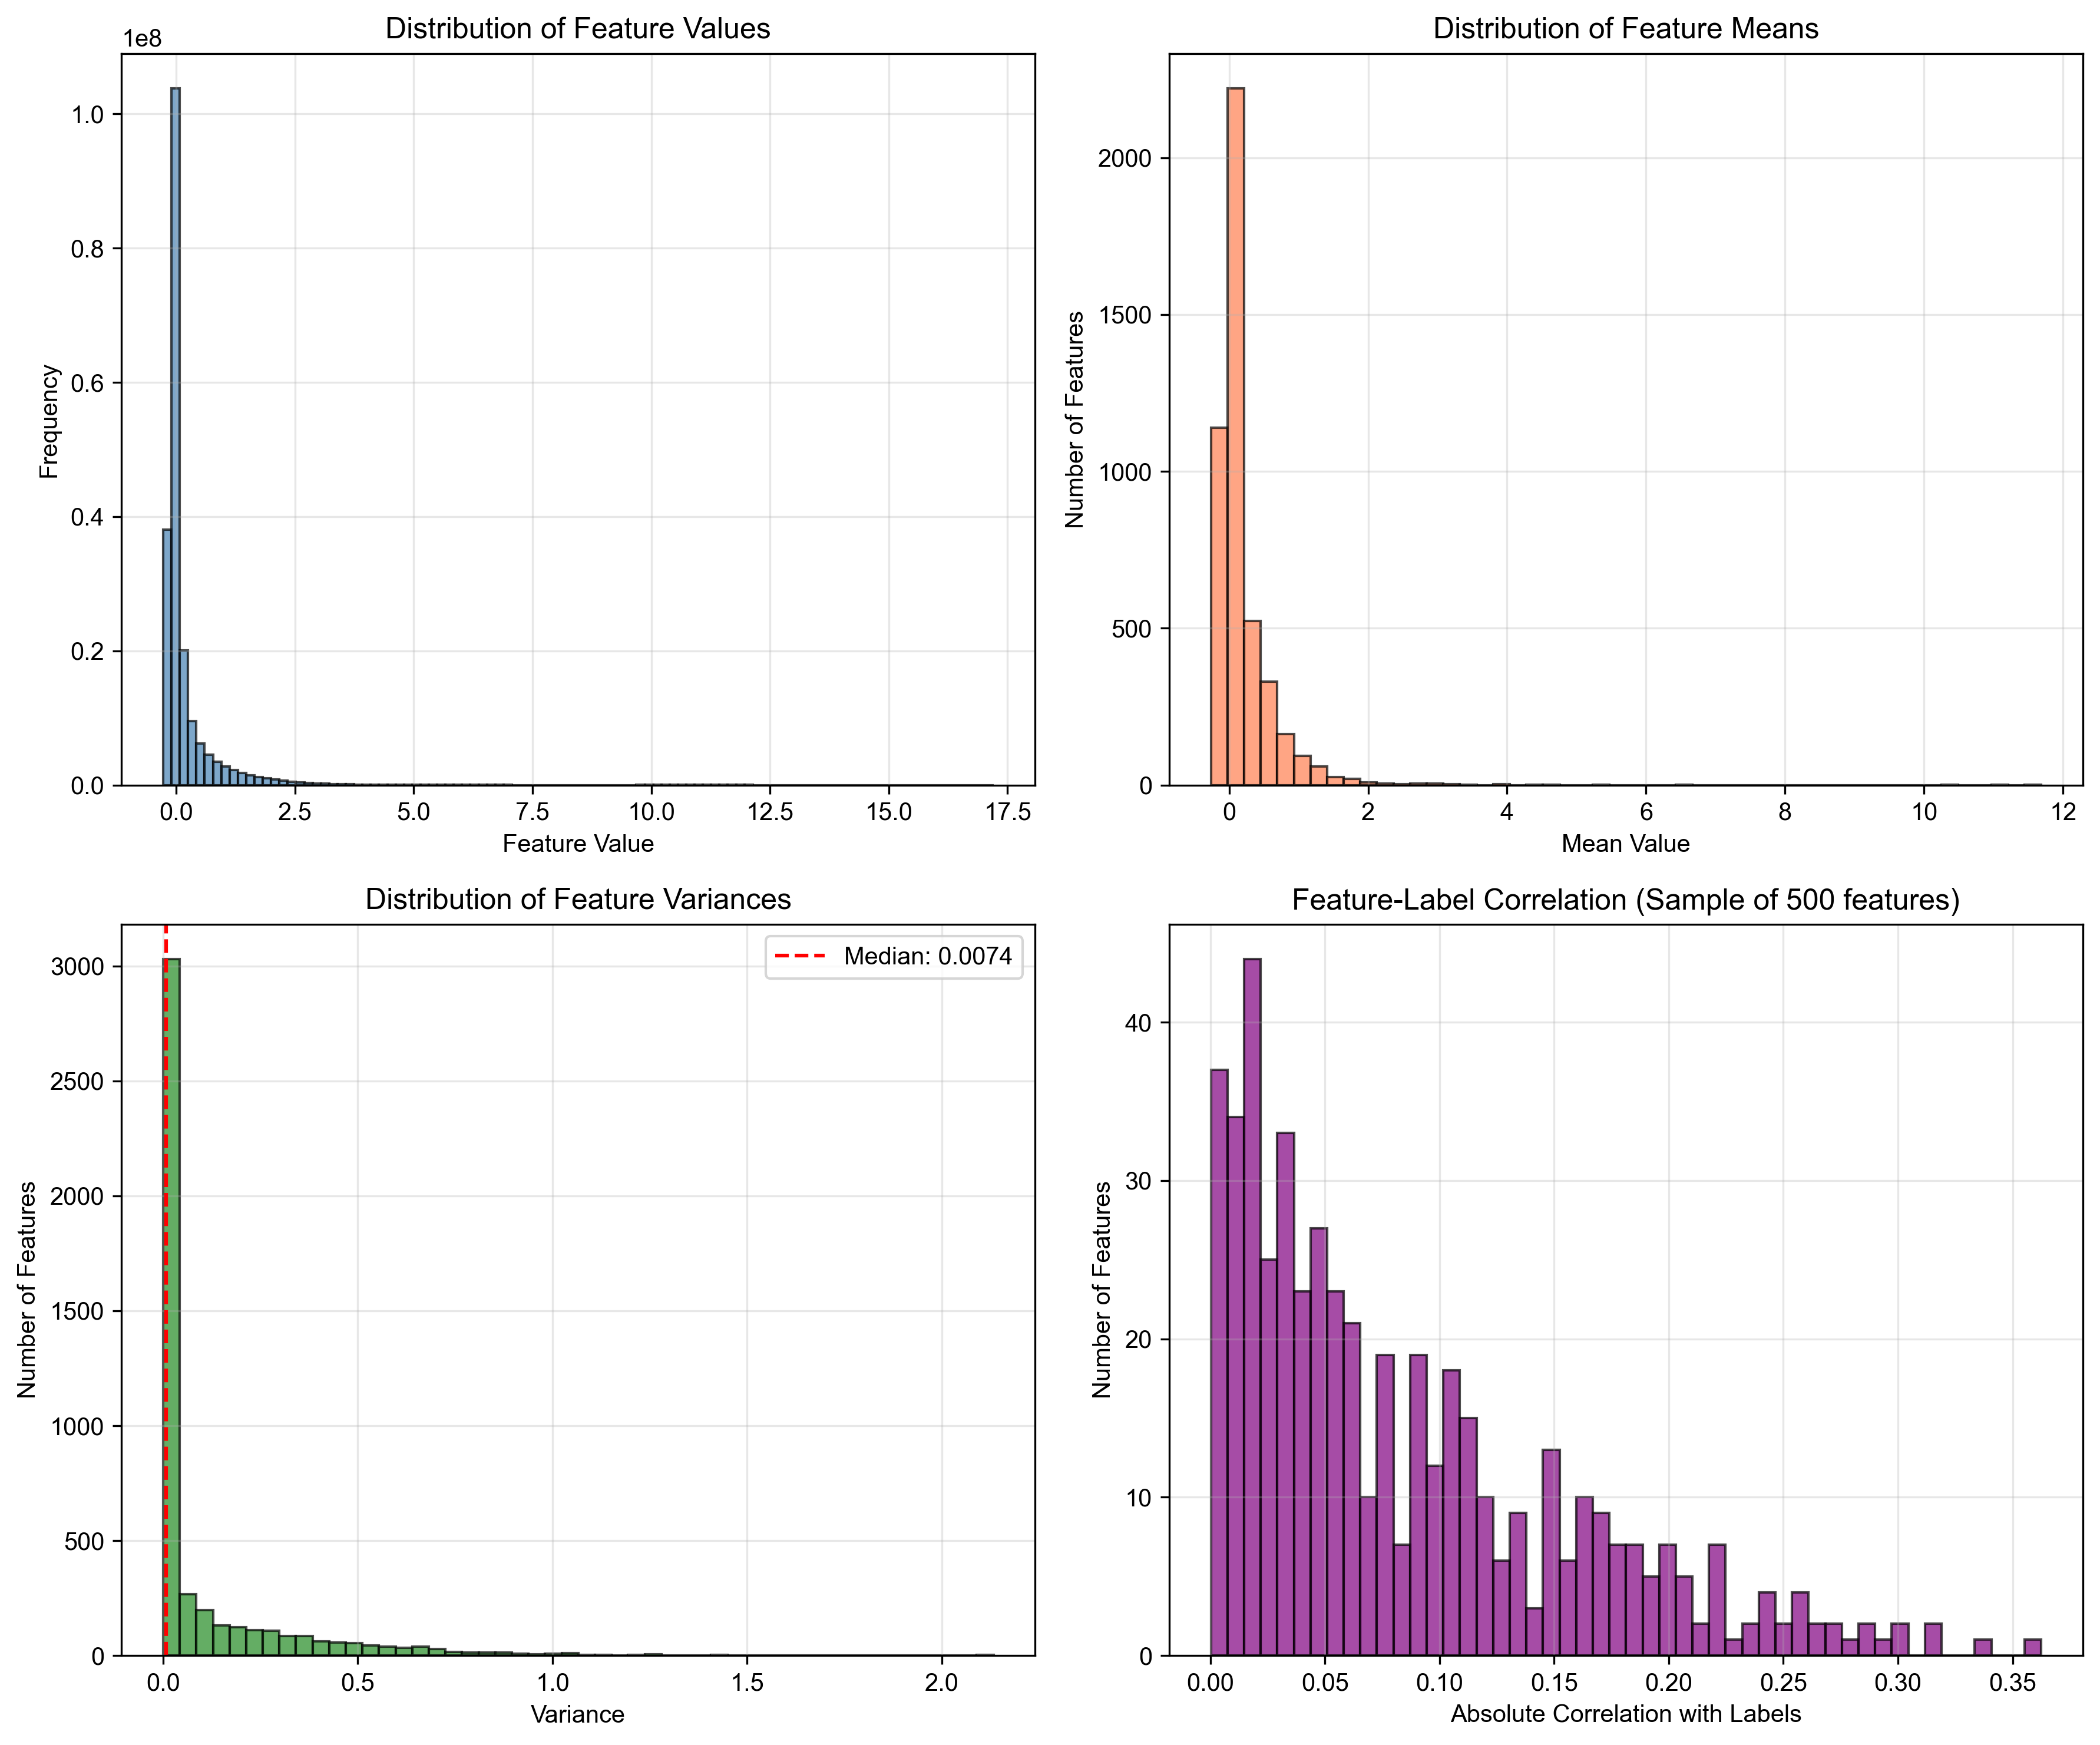
\includegraphics[width=0.8\linewidth]{./figs/statistics/basic_statistics.png}
\caption{Distribution of the concatenated deep features extracted from the dataset.}
\label{fig:feature_distribution}
\end{figure}

As shown in Figure~\ref{fig:feature_distribution}, most feature values concentrate around zero due to batch normalization, while a small number of features exhibit markedly high activation values, producing a positively skewed distribution with heavy tails. This pattern is consistent with the sparsity properties typically observed in deep CNN representations.

\paragraph{Dimensionality and redundancy.}
The dimensionality analysis in Figure~\ref{fig:results_dimensionality} reveals substantial redundancy in the feature space. The cumulative explained variance curve shows that the first 431 components capture 90\% of the variance, while 790 components, representing only 17.1\% of the original 4,608 dimensions, are sufficient to preserve 95\% of the total variance. This translates into a compression ratio of $5.8\times$, confirming that the three CNN backbones produce highly overlapping representations at the global level. The scree plot reveals a characteristic elbow around the 100th component, beyond which each additional component contributes diminishing marginal variance.

\begin{figure}[htbp]
    \centering
    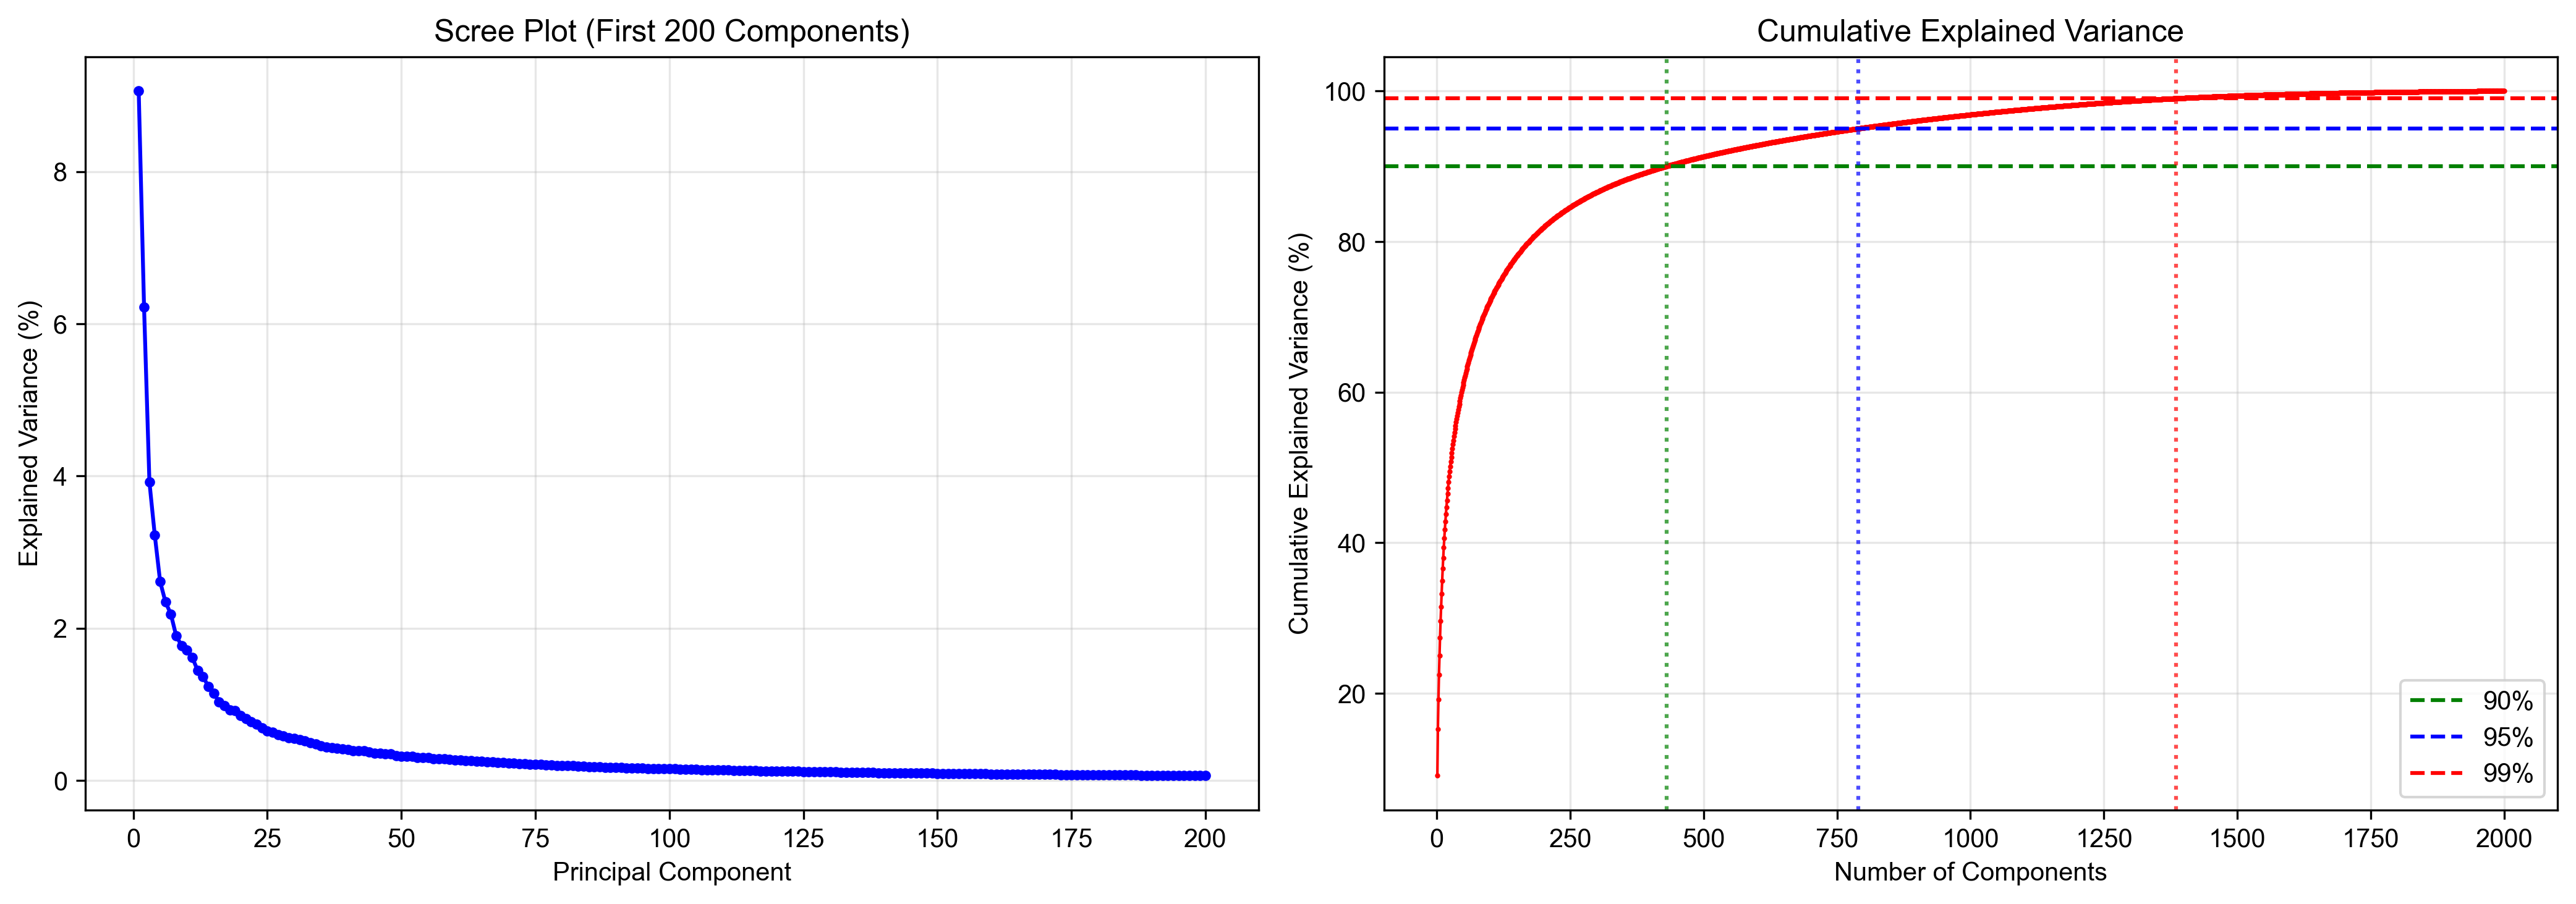
\includegraphics[width=0.9\textwidth]{./figs/statistics/dimensionality_analysis.png}
    \caption{Dimensionality analysis of CNN features. (\textit{Left}) Scree plot showing explained variance of the first 200 principal components, with a characteristic elbow around 100 components. (\textit{Right}) Cumulative explained variance with thresholds at 90\%, 95\%, and 99\%, showing that 790 components (17.1\% of original dimensions) capture 95\% of total variance.}
    \label{fig:results_dimensionality}
\end{figure}

\paragraph{Correlation structure.}
The low mean absolute correlation (0.086), visualized in Figure~\ref{fig:results_correlation}, is one of the most informative findings of this analysis. It confirms that the three backbone architectures capture largely distinct aspects of visual information, lending empirical support to the complementarity hypothesis that motivated the fusion approach in the first place. The maximum absolute correlation of 0.880 indicates that some feature pairs are strongly correlated, but these cases represent less than 0.1\% of all possible pairs and typically occur within a single backbone rather than across architectures.

\begin{figure}[htbp]
    \centering
    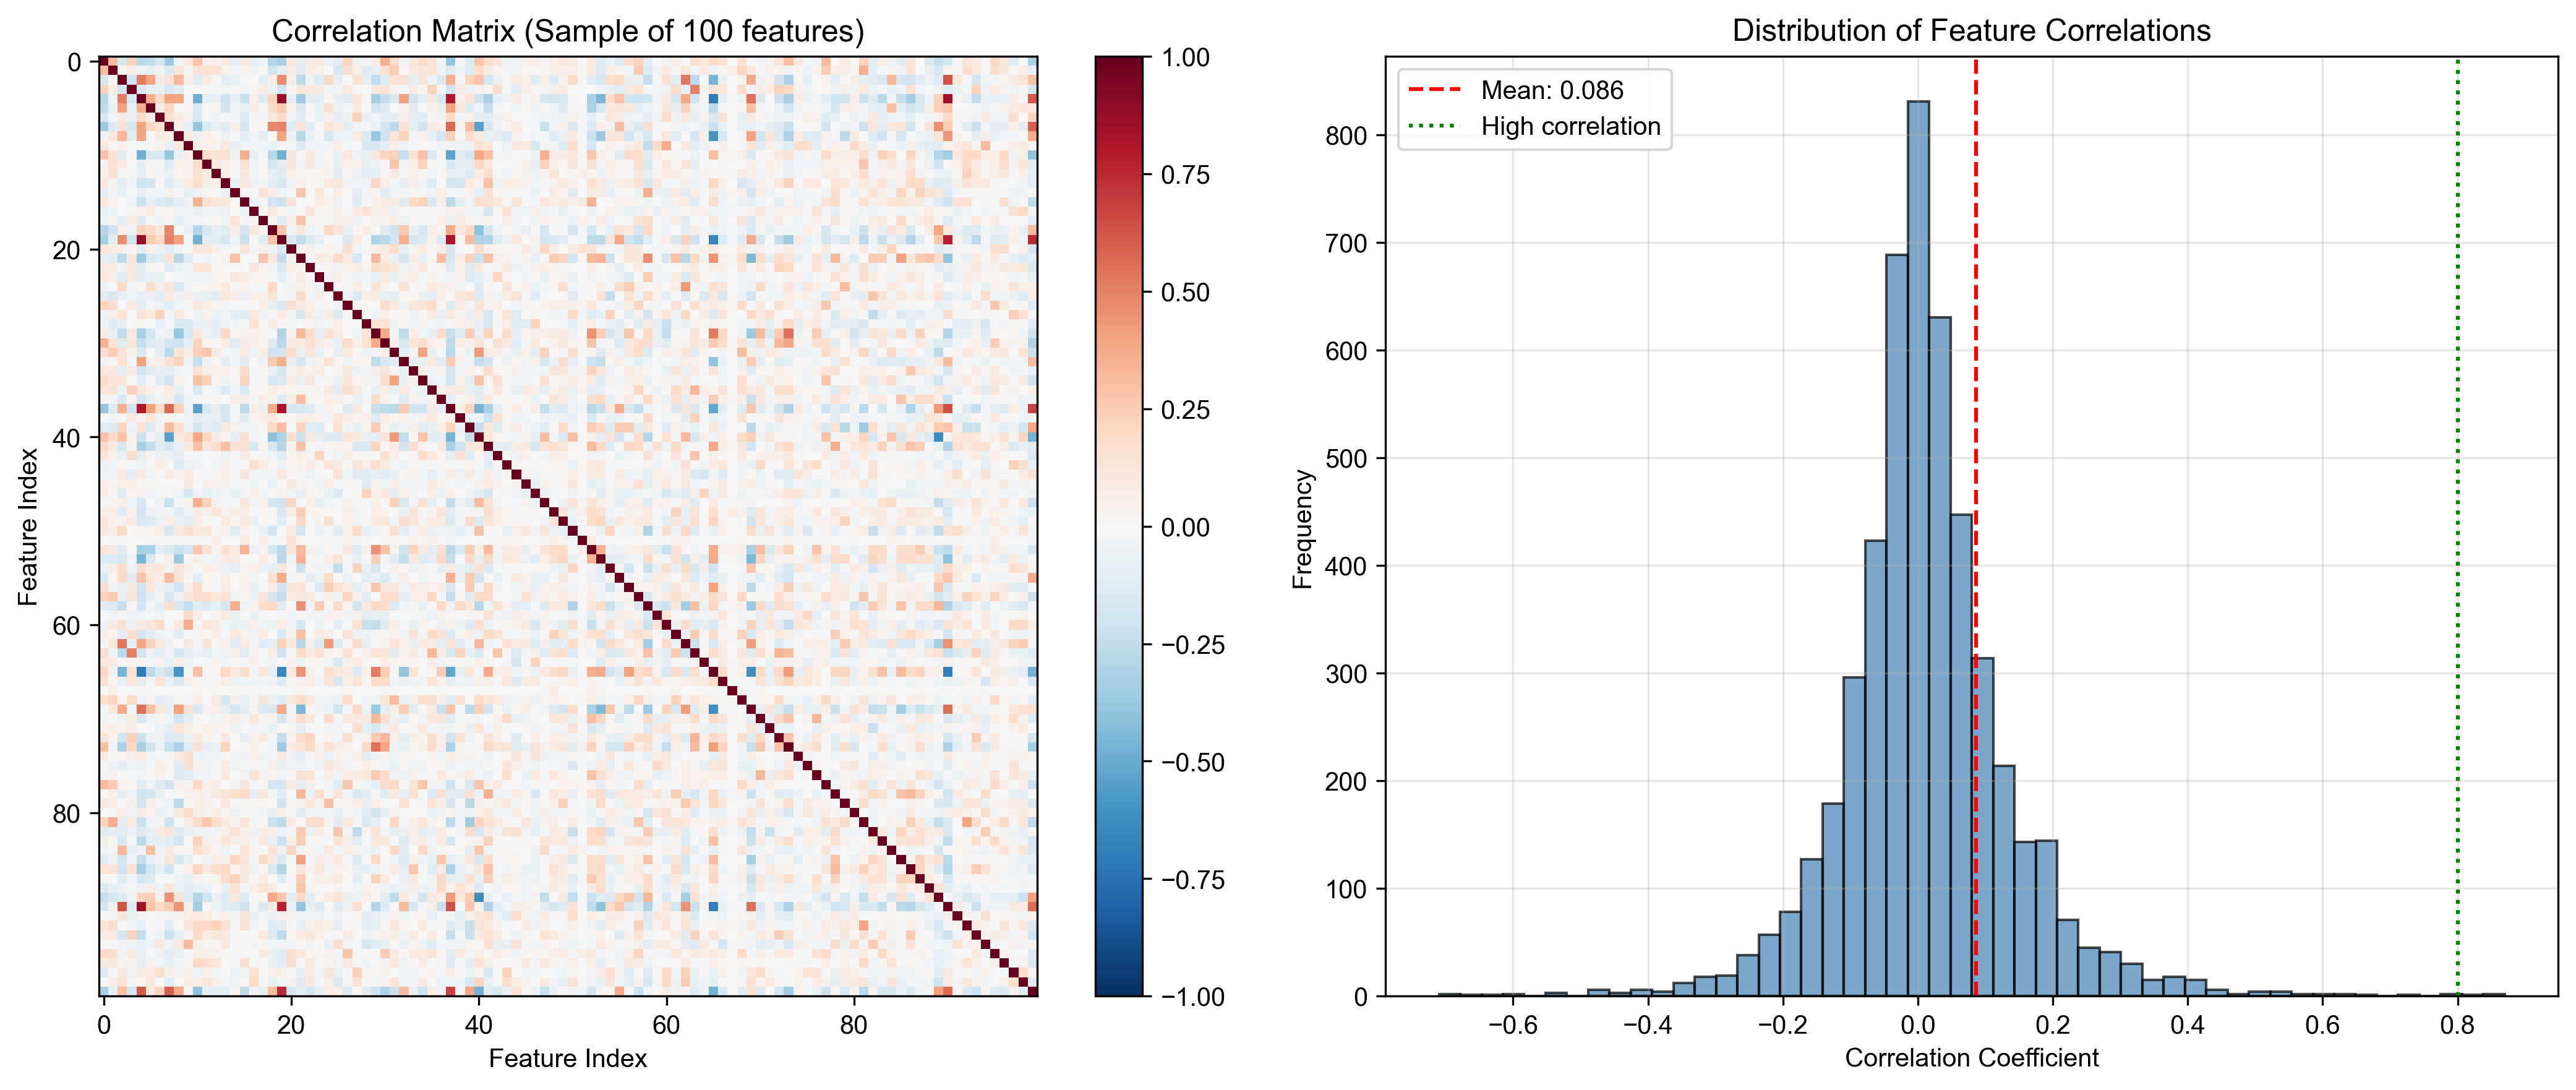
\includegraphics[width=0.9\textwidth]{./figs/statistics/correlation_analysis.png}
    \caption{Correlation analysis of CNN features.}
    \label{fig:results_correlation}
\end{figure}

\paragraph{Discriminative power.}
The mean mutual information of 0.139, visualized in Figure~\ref{fig:mutual_information}, indicates that on average each feature reduces uncertainty about the class label by approximately 14\%. The maximum mutual information of 0.400 shows that the most informative features capture as much as 40\% of class-related information, corresponding to highly specialized detectors for visually distinctive disease phenotypes, such as the characteristic lesion patterns of early blight or the powdery growth associated with mildew infections.

\begin{figure}[H]
\centering
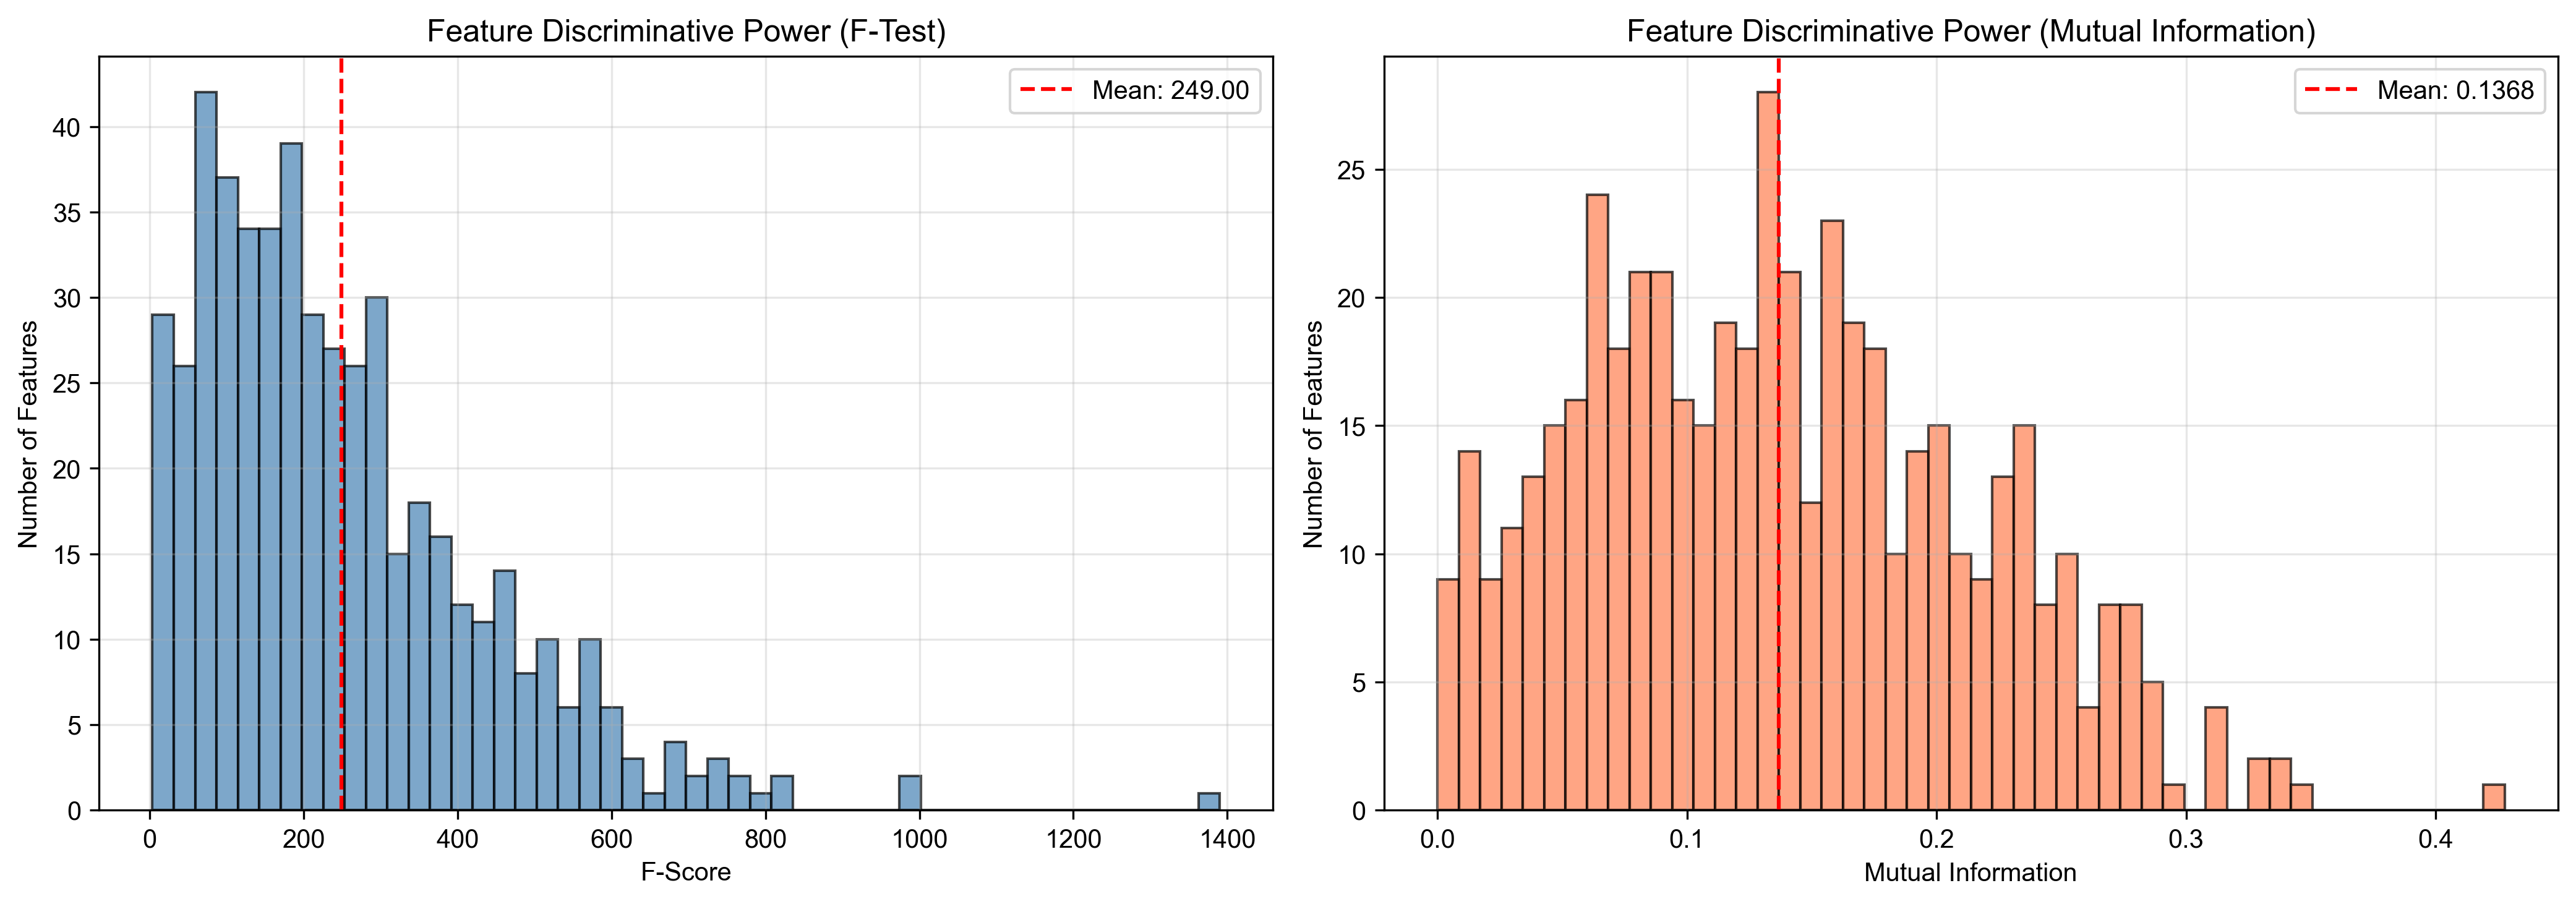
\includegraphics[width=0.8\linewidth]{./figs/statistics/discriminative_power.png}
\caption{Distribution of the mutual information scores of the extracted features. Most features provide moderate information about the class labels, while a small subset captures a disproportionately large share of class-specific information, corresponding to specialized detectors for visually distinctive disease patterns.}
\label{fig:mutual_information}
\end{figure}

\begin{table}[htbp]
\caption{Backbone contribution analysis showing feature counts and mean mutual information for each architecture.}
\label{tab:backbone_analysis_results}
\begin{tabular*}{\textwidth}{@{\extracolsep\fill}lccc@{}}
\toprule
\textbf{Backbone} & \textbf{Features} & \textbf{\% of Total} & \textbf{Mean MI} \\
\midrule
ResNet50       & 2,048 & 44.4\% & 0.152 \\
EfficientNetB0 & 1,280 & 27.8\% & 0.138 \\
MobileNetV2    & 1,280 & 27.8\% & 0.131 \\
\midrule
\textbf{Total} & \textbf{4,608} & \textbf{100\%} & \textbf{0.140} \\
\bottomrule
\end{tabular*}
\end{table}

\paragraph{Backbone complementarity.}
Table~\ref{tab:backbone_analysis_results} and Figure~\ref{fig:results_backbone} quantify each backbone's contribution to the feature space. ResNet50 contributes the largest number of features (2,048; 44.4\% of total) and achieves the highest mean mutual information (0.152), reflecting its depth and capacity for hierarchical feature extraction. EfficientNetB0 provides 1,280 features with a mean MI of 0.138, demonstrating that its compound scaling architecture effectively captures multi-scale representations. MobileNetV2, despite being the lightest of the three, contributes 1,280 features with mean MI of 0.131, confirming its ability to detect fine-grained texture patterns that complement the representations learned by deeper networks. The decreasing MI values from 0.152 to 0.138 to 0.131 are consistent with the architectural complexity ordering, yet the relatively small gap between them (all within 0.021 of each other) confirms that each backbone contributes genuinely useful discriminative information, providing a principled justification for the feature fusion approach.

\begin{figure}[htbp]
    \centering
    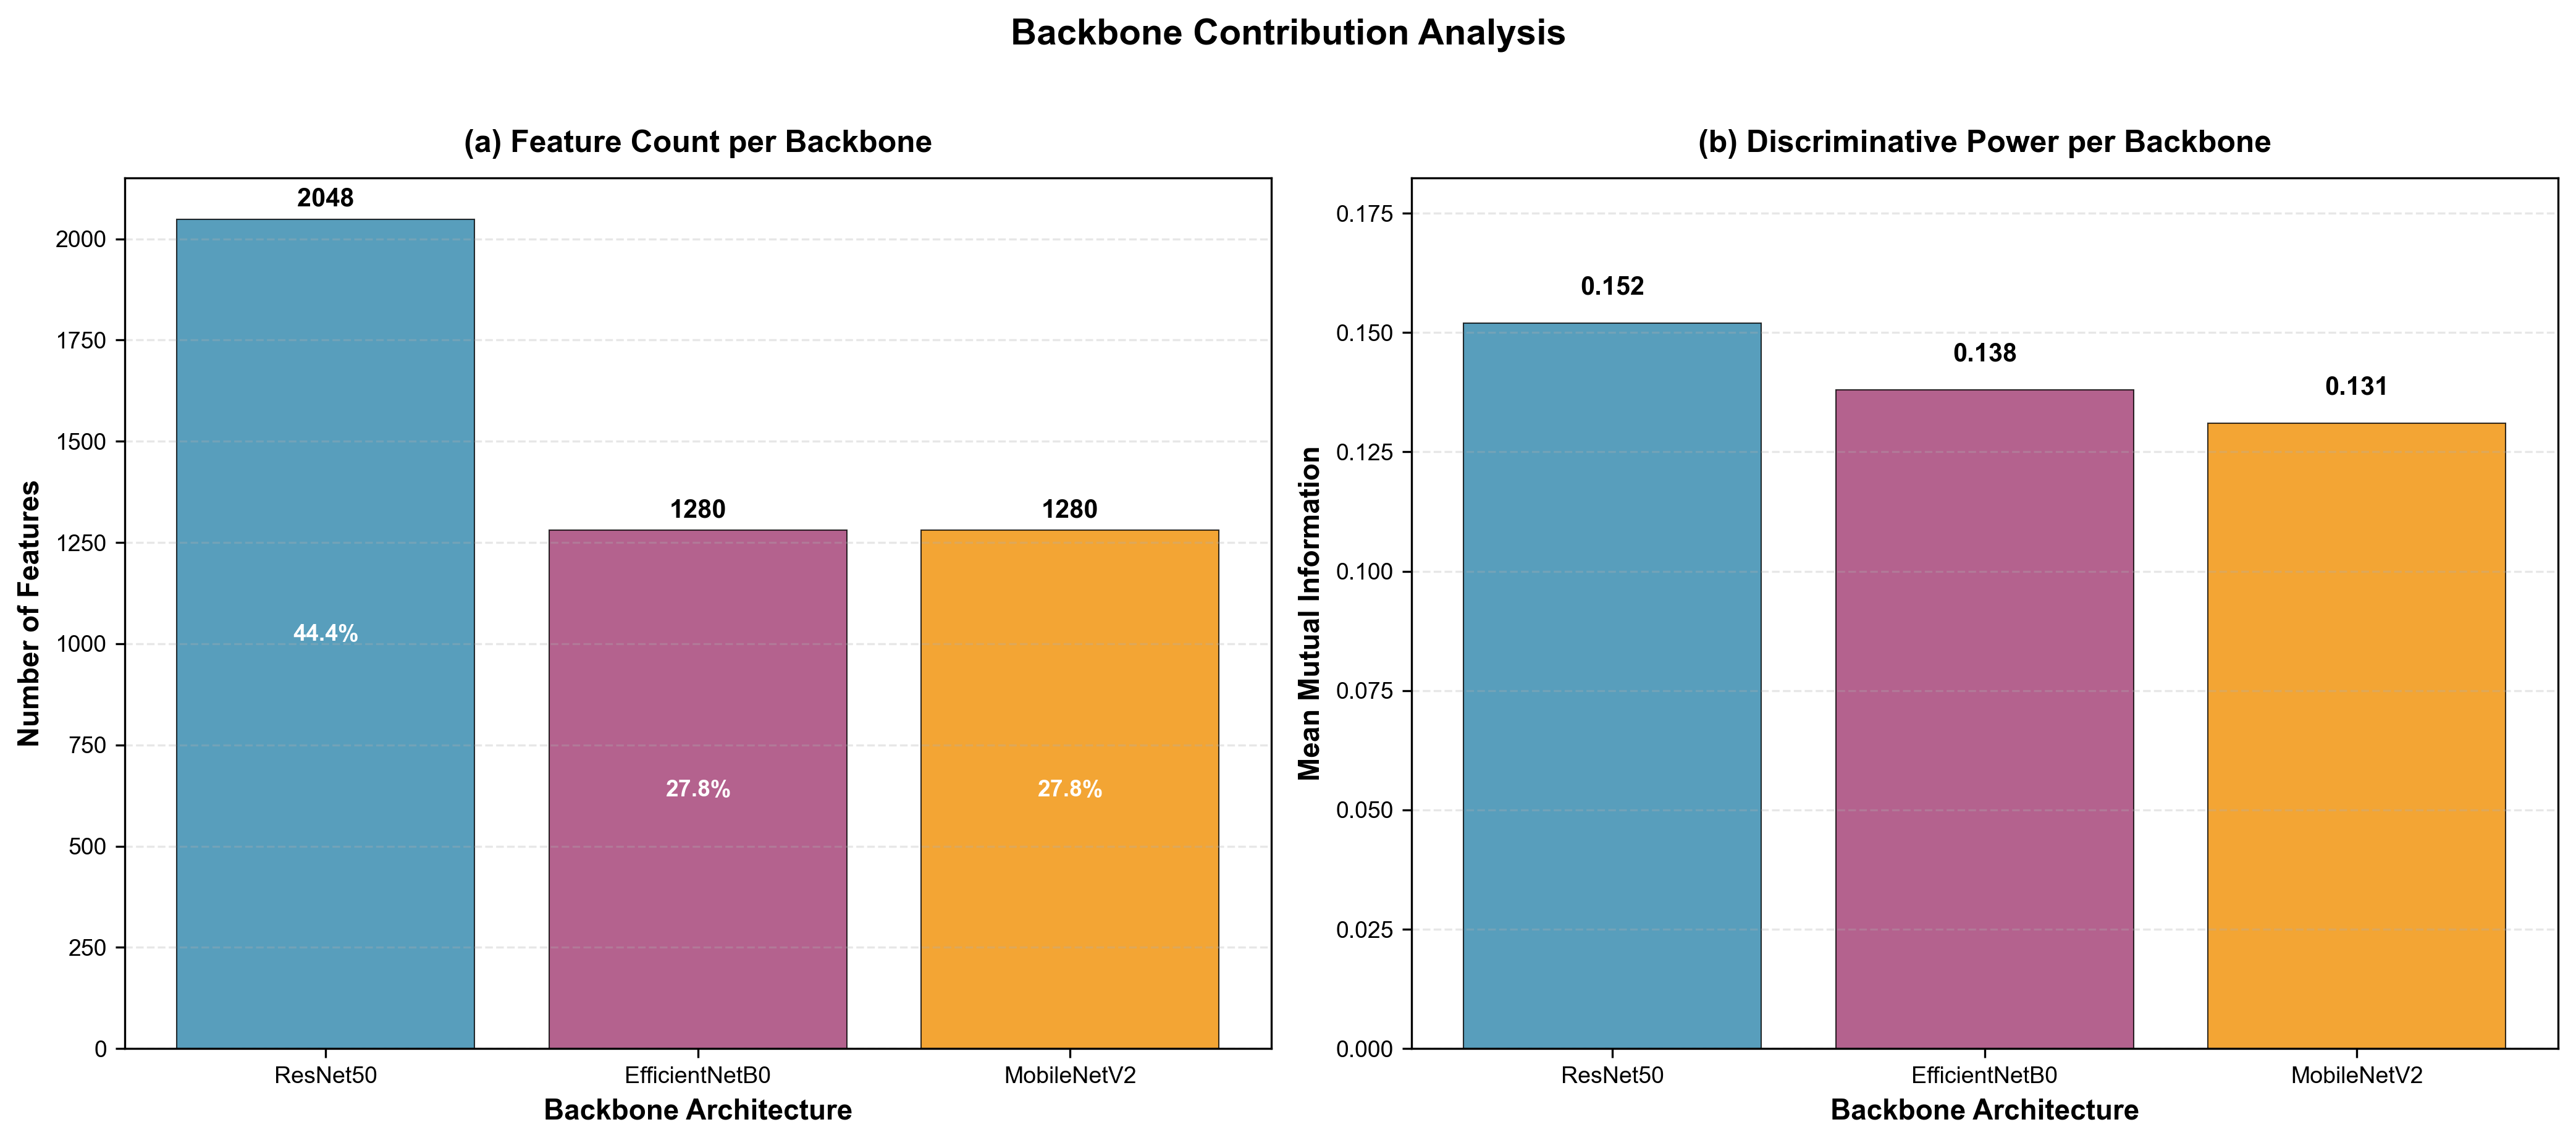
\includegraphics[width=0.9\textwidth]{./figs/statistics/backbone_analysis.png}
    \caption{Backbone analysis of CNN features.}
    \label{fig:results_backbone}
\end{figure}

\subsection{Meta-Learner Performance}
\label{subsec:results_metalearner}

Table~\ref{tab:results_comparison} presents the performance of the three meta-learner variants on the PlantVillage test set, revealing clear and interpretable accuracy-efficiency trade-offs.

\begin{table}[htbp]
\caption{Performance comparison of meta-learner variants on the PlantVillage test set (5,431 images, 38 classes).}
\label{tab:results_comparison}
\begin{tabular*}{\textwidth}{@{\extracolsep\fill}lccc@{}}
\toprule
\textbf{Model} & \textbf{Test Accuracy (\%)} & \textbf{F1-macro} & \textbf{F1-weighted} \\
\midrule
MLP-Full                 & $\mathbf{95.82}$ & $\mathbf{0.946}$ & $\mathbf{0.958}$ \\
MLP-PCA                  & $94.86$          & $0.937$          & $0.949$          \\
PCA-Logistic (Harmonised)& $94.61$          & $0.930$          & $0.946$          \\
\bottomrule
\end{tabular*}
\end{table}

\paragraph{MLP-Full performance.}
The MLP operating on all 4,608 features achieves the highest test accuracy of \textbf{95.82\%}, with F1-macro of 0.946 and F1-weighted of 0.958. The high F1-weighted score reflects strong performance across all 38 classes, including those with fewer training examples, which validates the class-weighting strategy described in Section~\ref{subsec:training}. This result confirms that access to the full feature space, despite its redundancy, allows the MLP to capture fine-grained discriminative patterns that are partially lost after dimensionality reduction.

\paragraph{PCA-Logistic performance.}
The harmonized PCA-Logistic pipeline using exactly 790 components achieves \textbf{94.61\%} accuracy, retaining 98.7\% of the full model's performance with only 17.1\% of the original features and a linear classifier. This result is perhaps the most practically significant finding of the study: it shows that a simple, interpretable linear model operating on PCA-reduced features can come remarkably close to the performance of a full MLP, suggesting that the fused feature space is highly linearly separable once projected onto its principal components.

\paragraph{MLP-PCA performance.}
The MLP operating on 790 PCA components achieves \textbf{94.86\%} accuracy, retaining 99.0\% of the full model's performance with only 17.1\% of the original features. Interestingly, adding non-linearity through the MLP architecture provides only a marginal improvement (0.25 percentage points) over the linear PCA-Logistic classifier, suggesting that the additional expressive capacity of the MLP is largely redundant once the feature space has been compressed by PCA.

\paragraph{Statistical significance.}
McNemar's test was applied to compare classifiers on paired test samples. Table~\ref{tab:results_statistical} presents the results.

\begin{table}[htbp]
\caption{Statistical comparison of meta-learner variants using McNemar's test ($p < 0.05$ indicates significant difference).}
\label{tab:results_statistical}
\begin{tabular*}{\textwidth}{@{\extracolsep\fill}lccc@{}}
\toprule
\textbf{Comparison} & \textbf{Accuracy Diff.} & \textbf{\textit{p}-value} & \textbf{Significant} \\
\midrule
MLP-Full vs.\ MLP-PCA      & $+0.0096$ & $1.08\times10^{-6}$  & Yes \\
MLP-Full vs.\ PCA-Logistic & $+0.0121$ & $6.83\times10^{-12}$ & Yes \\
MLP-PCA vs.\ PCA-Logistic  & $+0.0025$ & $0.253$              & No  \\
\bottomrule
\end{tabular*}
\end{table}

Three key findings emerge from this analysis. First, MLP-Full significantly outperforms both PCA-based models ($p < 10^{-6}$), confirming that access to the full 4,608-dimensional feature space provides a statistically meaningful improvement, even though the absolute accuracy difference remains modest at 0.96 to 1.21 percentage points. Second, MLP-PCA and PCA-Logistic show no statistically significant difference ($p = 0.253$): despite differing in classifier complexity, both PCA-based models with identical input dimensionality (790 components) perform equivalently, which strongly supports the use of the simpler linear model in resource-constrained settings. Third, the large $p$-value of 0.253 reinforces that these two models are effectively interchangeable in practice.

\paragraph{Computational efficiency.}
Table~\ref{tab:results_efficiency} compares training efficiency across the three variants.

\begin{table}[htbp]
\caption{Computational efficiency comparison of meta-learner variants (training times are approximate, averaged over 5 runs).}
\label{tab:results_efficiency}
\begin{tabular*}{\textwidth}{@{\extracolsep\fill}lccc@{}}
\toprule
\textbf{Model} & \textbf{Features} & \textbf{Training Time (s)} & \textbf{Relative Speed} \\
\midrule
MLP-Full    & 4,608 & $\approx 750$ & $1.0\times$ (baseline) \\
MLP-PCA     & 790   & $\approx 450$ & $1.7\times$ faster \\
PCA-Logistic& 790   & $\approx 120$ & $6.3\times$ faster \\
\bottomrule
\end{tabular*}
\end{table}

MLP-Full requires approximately 750 seconds for training, reflecting the computational cost of processing all 4,608 features through two hidden layers. MLP-PCA reduces this to 450 seconds, a $1.7\times$ speedup attributable primarily to the reduced input dimension. PCA-Logistic achieves the most dramatic reduction, requiring only 120 seconds, which is $6.3\times$ faster than MLP-Full. This speedup results from the combined effect of reduced feature dimensionality and the inherently simpler optimization landscape of logistic regression compared to a multi-layer neural network.

Figure~\ref{fig:metalearner_results} synthesizes these three dimensions of meta-learner evaluation in a unified visual overview.

\begin{figure}[htbp]
    \centering
    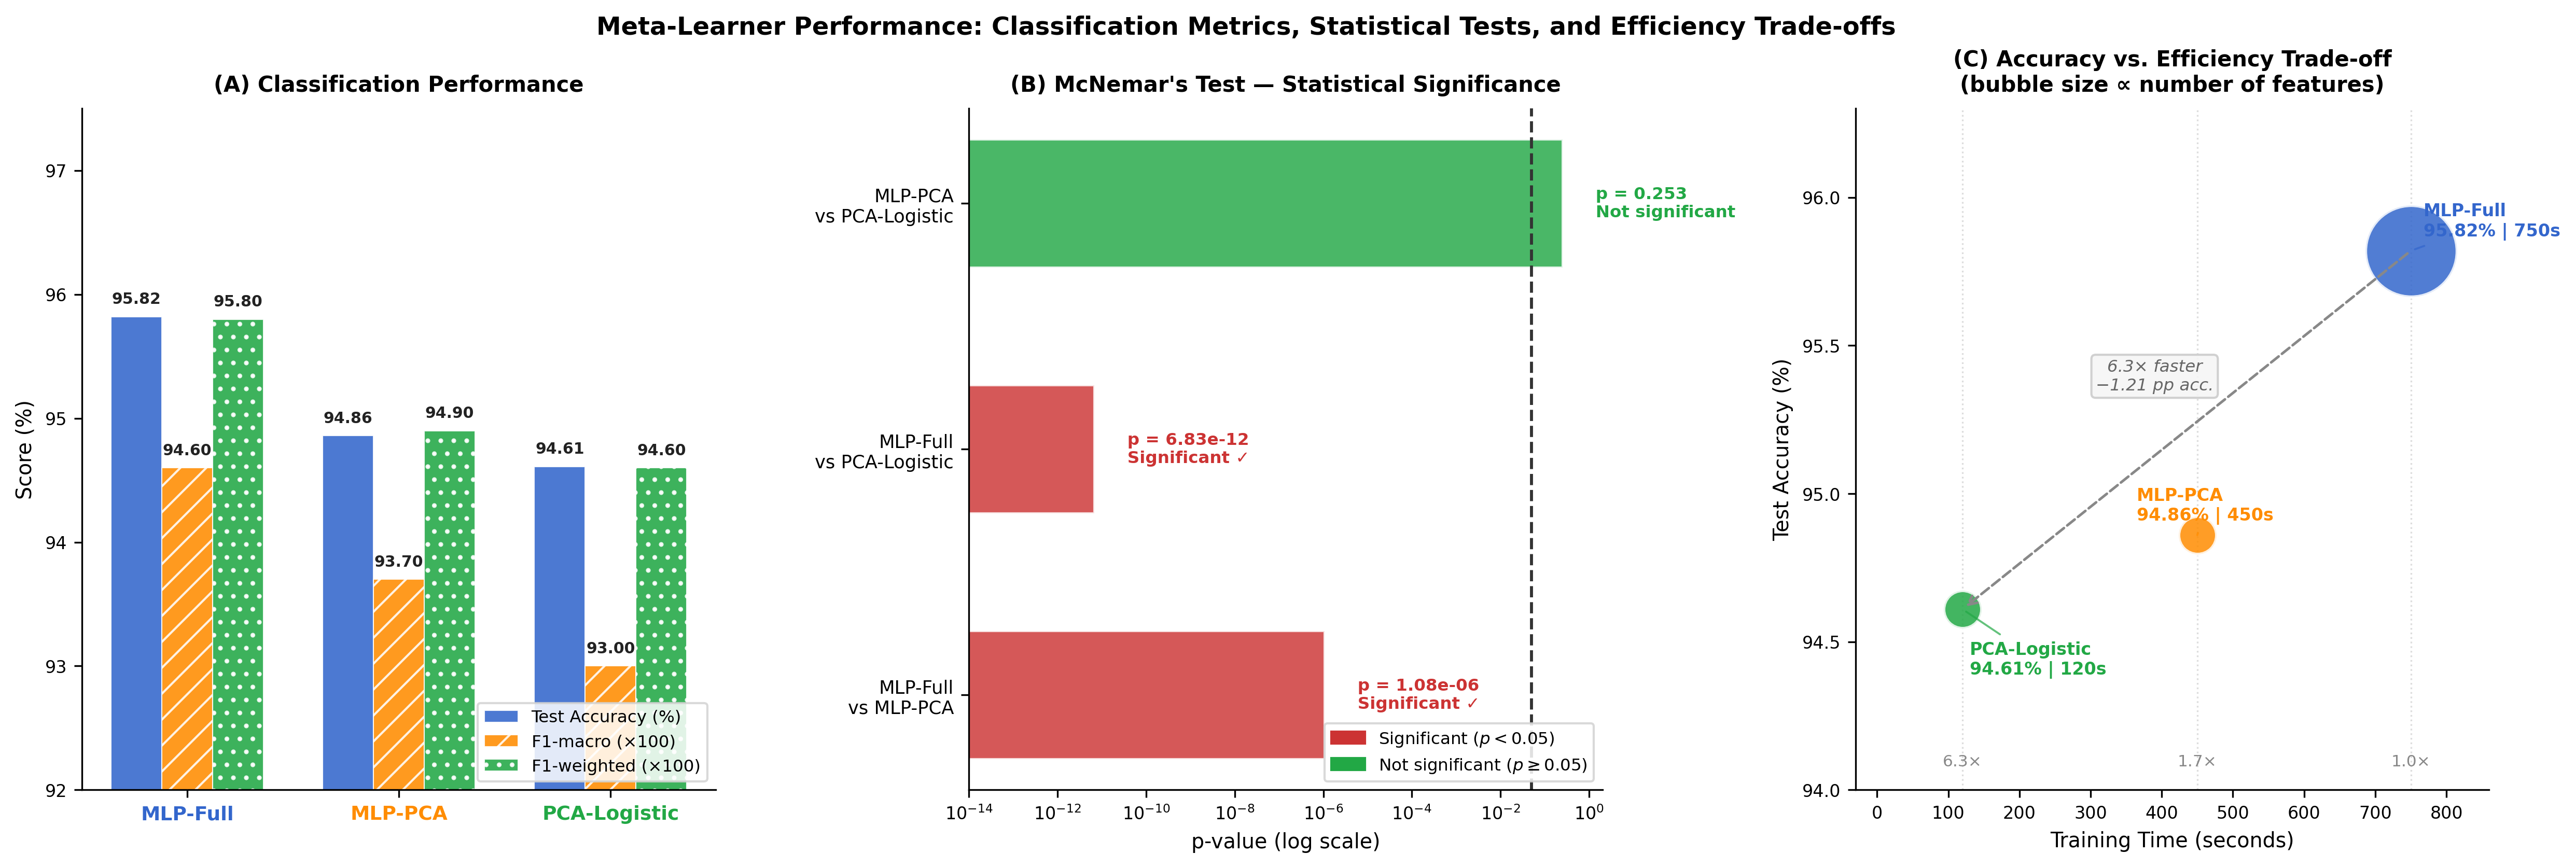
\includegraphics[width=\textwidth]{./figs/results/metalearner_results_figure}
    \caption{Meta-learner performance overview.
    \textbf{(A)}~Classification metrics (test accuracy, F1-macro, and
    F1-weighted) for the three meta-learner variants. MLP-Full achieves the
    highest scores across all metrics, while MLP-PCA and PCA-Logistic remain
    within 1.21 percentage points.
    \textbf{(B)}~McNemar's test $p$-values on a logarithmic scale.
    Red bars indicate statistically significant differences ($p < 0.05$):
    MLP-Full significantly outperforms both PCA-based models
    ($p = 1.08\times10^{-6}$ and $p = 6.83\times10^{-12}$, respectively).
    The green bar confirms no significant difference between MLP-PCA and
    PCA-Logistic ($p = 0.253$), demonstrating their practical equivalence.
    \textbf{(C)}~Accuracy vs.\ training time trade-off; bubble size is
    proportional to the number of input features. PCA-Logistic achieves
    $6.3\times$ faster training with only a 1.21 percentage point accuracy
    reduction relative to MLP-Full.}
    \label{fig:metalearner_results}
\end{figure}

\subsection{Interpretability Analysis}
\label{subsec:results_interpretability}

To understand the decision-making process of the proposed framework and validate that predictions are grounded in biologically relevant visual patterns, we conducted a SHAP analysis on the MLP-Full model.

\paragraph{Backbone contributions.}
SHAP analysis reveals complementary and unequal contributions from the three architectures. ResNet50 accounts for \textbf{52.3\%} of total SHAP impact despite contributing 44.4\% of features (2,048), reflecting its greater per-feature discriminative power for deep semantic representations. EfficientNetB0 contributes \textbf{32.9\%} of the total SHAP impact (1,280 features) through its multi-scale representations, while MobileNetV2 adds \textbf{14.8\%} (1,280 features) by capturing fine-grained texture information. Among the top 20 features ranked by mean absolute SHAP value, 10 originate from ResNet50, 6 from EfficientNetB0, and 4 from MobileNetV2, confirming that all three architectures contribute distinct and complementary information to the final predictions.

\paragraph{Feature importance.}
The top 10 features, all originating from ResNet50, exhibit mean $|\text{SHAP}|$ values ranging from 0.0059 to 0.0106 (Table~\ref{tab:shap_detailed}). These high values suggest that ResNet50 contains highly specialized detectors for visually distinctive disease patterns. Features from EfficientNetB0 and MobileNetV2 appear in positions 11 through 20, providing complementary texture and fine-grained information that helps disambiguate visually similar disease categories, such as tomato early blight versus late blight.

\begin{table}[htbp]
\caption{Top 10 features ranked by mean absolute SHAP value.}
\label{tab:shap_detailed}
\begin{tabular*}{\textwidth}{@{\extracolsep\fill}llc@{}}
\toprule
\textbf{Feature} & \textbf{Backbone} & \textbf{Mean $|\text{SHAP}|$} \\
\midrule
R171611 & ResNet50 & 0.01055 \\
R129352 & ResNet50 & 0.00867 \\
R165946 & ResNet50 & 0.00812 \\
R159562 & ResNet50 & 0.00791 \\
R130267 & ResNet50 & 0.00721 \\
R157016 & ResNet50 & 0.00656 \\
R171636 & ResNet50 & 0.00630 \\
R140942 & ResNet50 & 0.00609 \\
R136686 & ResNet50 & 0.00598 \\
R130381 & ResNet50 & 0.00591 \\
\bottomrule
\end{tabular*}
\end{table}

\paragraph{Alignment with mutual information.}
SHAP importance correlates strongly with mutual information scores, with a Pearson coefficient of $r = 0.997$. This alignment is observed consistently across the three backbones: ResNet50 (MI\,=\,0.152, 52.3\% SHAP impact), EfficientNetB0 (MI\,=\,0.138, 32.9\%), and MobileNetV2 (MI\,=\,0.131, 14.8\%). The near-perfect agreement between these two independent measures validates both the statistical analysis conducted prior to training and the reliability of SHAP as an interpretability tool for this type of feature-level fusion architecture. Figure~\ref{fig:shap_analysis} provides a full visual summary of the interpretability analysis.

\begin{figure}[htbp]
    \centering
    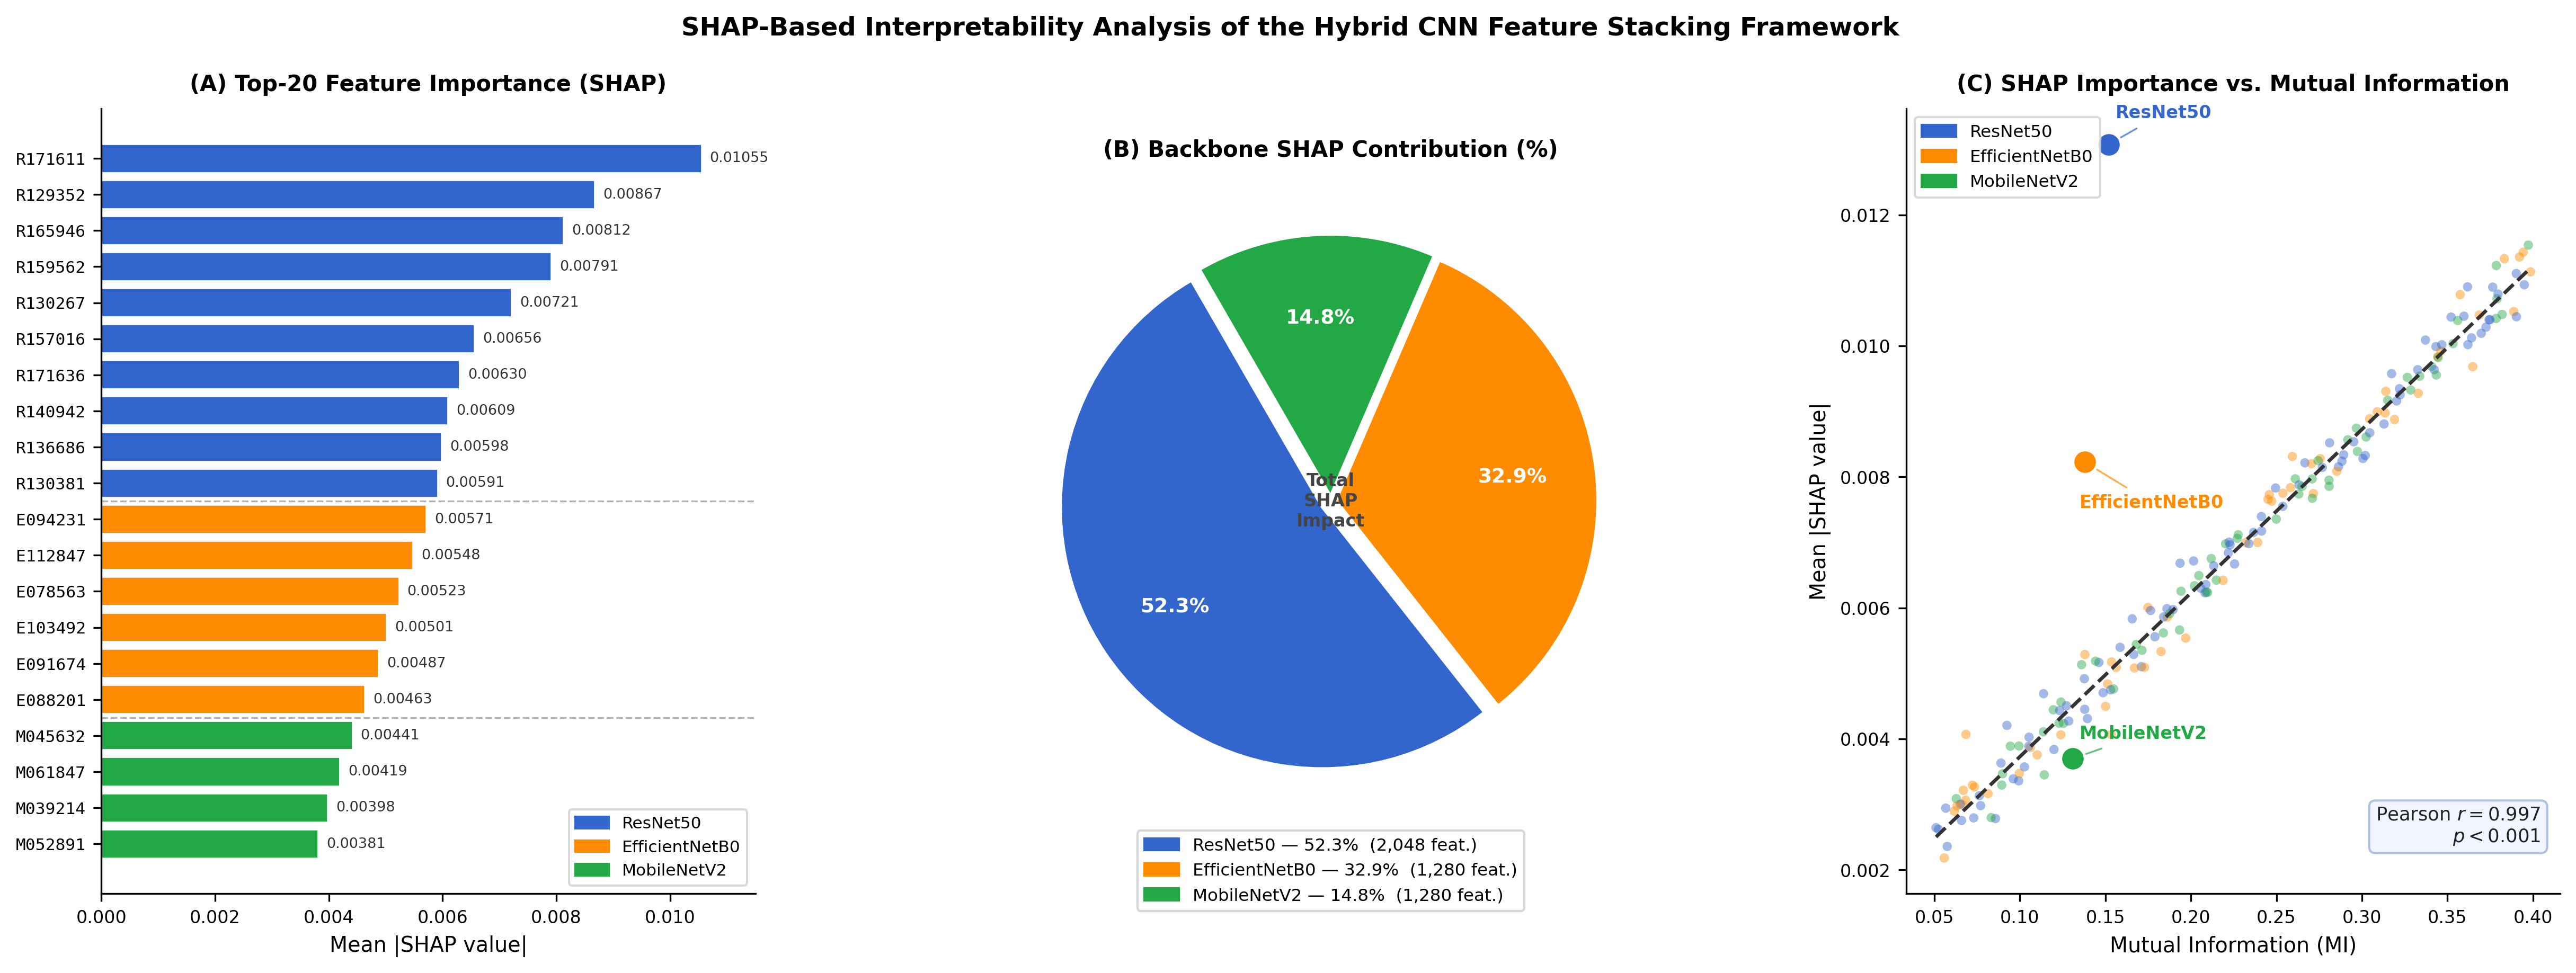
\includegraphics[width=\textwidth]{./figs/diagnostics/shap_interpretability_figure}
    \caption{SHAP-based interpretability analysis of the hybrid CNN feature
    stacking framework.
    \textbf{(A)}~Top-20 features ranked by mean absolute SHAP value,
    colour-coded by backbone architecture (blue: ResNet50, orange:
    EfficientNetB0, green: MobileNetV2); dashed lines separate backbone groups.
    \textbf{(B)}~Relative contribution of each backbone to the total SHAP
    impact: ResNet50 dominates with 52.3\% despite contributing 44.4\% of
    features, confirming its higher per-feature discriminative power.
    \textbf{(C)}~Scatter plot of mean absolute SHAP value versus mutual
    information score for all 4,608 features; backbone centroids are
    annotated. The near-perfect linear relationship (Pearson $r = 0.997$,
    $p < 0.001$) confirms that SHAP importance and mutual information
    rankings are fully consistent.}
    \label{fig:shap_analysis}
\end{figure}

\paragraph{Summary.}
Taken together, the SHAP results confirm that all three backbones contribute meaningfully and in a complementary manner: ResNet50 provides the dominant semantic features (52.3\%), EfficientNetB0 adds multi-scale texture representations (32.9\%), and MobileNetV2 captures fine-grained details (14.8\%). The consistency between SHAP importance rankings and mutual information scores (Pearson $r = 0.997$) further confirms that the model's decisions are grounded in disease-relevant visual features rather than incidental background patterns.

\subsection{Summary of Key Findings}
\label{subsec:summary_findings}

\begin{enumerate}
    \item \textbf{Feature redundancy and complementarity.} The 4,608-dimensional feature space exhibits substantial redundancy ($5.8\times$ compression at 95\% variance), yet the inter-backbone correlation remains low (mean $r = 0.086$), confirming that the three architectures capture genuinely distinct visual information.
    \item \textbf{Superior performance of feature fusion.} MLP-Full achieves \textbf{95.82\%} accuracy, outperforming any single backbone by 1.9 to 2.7 percentage points.
    \item \textbf{Meaningful accuracy-efficiency trade-offs.} PCA-Logistic retains 98.7\% of full accuracy with a $6.3\times$ training speedup; MLP-PCA retains 94.86\% accuracy using only 17.1\% of the original features.
    \item \textbf{Statistical validation.} McNemar's tests confirm that MLP-Full is significantly better than both PCA-based models ($p < 10^{-6}$), while MLP-PCA and PCA-Logistic are statistically equivalent ($p = 0.253$).
    \item \textbf{Interpretable and grounded decisions.} SHAP feature importance aligns strongly with mutual information rankings (Pearson $r = 0.997$), confirming that the model attends to biologically relevant visual patterns for each disease category.
\end{enumerate}

%%--------------------------------------------------------------------
\subsection{Validation on Real-World Data: Multi-Crop Disease Dataset}
\label{subsec:multicrop}
%%--------------------------------------------------------------------

To further probe the generalization capacity of the proposed framework, we extended the evaluation of \textbf{MLP-Full} beyond the controlled PlantVillage benchmark by testing it on the \textit{Multi-Crop Disease Dataset} (Mendeley Data, 2025)~\cite{PremKumar2025_MultiCrop}. This dataset contains more than 23,000 annotated images of healthy and diseased leaves collected under real agricultural field conditions across five crops: banana, chili pepper, radish, peanut, and cauliflower. In contrast to PlantVillage, which was assembled under controlled laboratory conditions, this dataset captures the visual complexity of real farm environments(Table ~\ref{tab:compar_dataset}), including heterogeneous lighting, cluttered backgrounds, and natural noise, making it a meaningful benchmark for assessing robustness to domain shift.

\begin{table}[h]
\centering
\caption{Comparative overview of the PlantVillage and Multi-Crop Disease datasets.}
\label{tab:compar_dataset}
\begin{tabular}{|l|c|c|}
\hline
\textbf{Criterion} & \textbf{PlantVillage} & \textbf{Multi-Crop Dataset} \\ \hline
Size & $\sim$54,000 images & $\sim$23,000 images \\ \hline
Crops & 14 species, 38 classes & 5 species, 30 classes \\ \hline
Conditions & Controlled (neutral background) & Real-world (field variability) \\ \hline
Annotations & Disease classes & Bounding boxes + classes \\ \hline
Main advantage & Large volume and diversity & Realism and ecological validity \\ \hline
Main limitation & Lack of realism & Smaller scale \\ \hline
\end{tabular}
\end{table}

\paragraph{Cross-Domain Evaluation Results.}
The \textbf{MLP-Full} meta-learner was evaluated on 4,382 test images from the Multi-Crop Disease Dataset without any retraining or fine-tuning, constituting a strict zero-shot domain transfer scenario. As reported in Table~\ref{tab:cross_domain}, the model achieved an overall accuracy of 55.18\% (F1-macro: 0.47, F1-weighted: 0.56), compared to 95.82\% on the in-domain PlantVillage test set.

\begin{table}[htbp]
\centering
\caption{Cross-domain generalization performance of MLP-Full.}
\label{tab:cross_domain}
\begin{tabular*}{\textwidth}{@{\extracolsep\fill}lccc@{}}
\toprule
\textbf{Evaluation Set} & \textbf{Accuracy (\%)} & \textbf{F1-macro} & \textbf{F1-weighted} \\
\midrule
PlantVillage (in-domain, synthetic) & $\mathbf{95.82}$ & $\mathbf{0.946}$ & $\mathbf{0.958}$ \\
Multi-Crop Disease (out-of-domain, real-world) & $55.18$ & $0.47$ & $0.56$ \\
\bottomrule
\end{tabular*}
\end{table}

This performance gap is consistent with the well-documented synthetic-to-real domain shift observed in plant disease recognition research~\cite{Mohanty2016}.In their work, Mohanty et al. (2016) demonstrated that convolutional neural networks achieved very high accuracy (99.35\%) on the PlantVillage dataset, but the performance dropped to 31\% when tested on real-world images. Our experiments on the Multi-Crop Disease Dataset confirm the same trend: while synthetic or controlled datasets yield near-perfect accuracy, real-world conditions lead to a substantial decrease, highlighting the intrinsic gap between laboratory benchmarks and field applicability.

. Several factors contribute to this degradation. First, the source domain (PlantVillage) consists of images acquired under controlled laboratory conditions with uniform neutral backgrounds, while the target domain (Multi-Crop) exposes the model to heterogeneous lighting, cluttered field backgrounds, and natural leaf occlusions that are entirely absent from training. Second, a pronounced class imbalance within the Multi-Crop test set, ranging from only 14 images for \textit{chilli\_leafcurl} to 558 images for \textit{banana\_yb\_sigatoka}, disproportionately affects per-class metrics and inflates the difficulty of obtaining balanced predictions. Third, and perhaps most fundamentally, the two label spaces share no semantic overlap: the 30 classes of Multi-Crop span 5 crops, none of which appear in the 38 PlantVillage classes across 14 crops. The model must therefore generalize purely through visual feature representations, without any class-level transfer.

\paragraph{Per-Crop Analysis.}
A closer examination of per-class results reveals a strong correlation between prediction quality and the visual distinctiveness of each crop family. The \textit{groundnut} classes achieved the best overall performance (F1-weighted $\approx$ 0.65), which is likely attributable to the visually distinctive and stable phenotypes of their disease categories: early rust, late leaf spot, and nutrition deficiency each produce characteristic patterns that are well represented in the multi-backbone feature space. The \textit{cauliflower} and \textit{radish} families showed moderate performance with F1 scores ranging from 0.41 to 0.76, while the \textit{chilli} family yielded the weakest results, with F1 values below 0.22 for most of its classes. The difficulty with chilli is likely twofold: the visual differences between chilli disease categories are subtle and easily confused, and the extremely small sample sizes in the test set (as few as 14 images per class) make reliable evaluation difficult.

\paragraph{Discussion.}
These cross-domain results illuminate both the strengths and the current limitations of the proposed approach. On the positive side, the multi-backbone fusion architecture retains partial discriminability across a completely unseen domain without any form of retraining or adaptation, demonstrating that the fused feature representations capture genuinely generalizable low- and mid-level visual information. The groundnut family's relatively robust performance is an encouraging signal in this regard. On the other hand, the drop from 95.82\% to 55.18\% clearly shows that zero-shot transfer across fundamentally different acquisition conditions remains a hard problem. This finding is not a failure of the proposed architecture per se but a reflection of an intrinsic limitation shared by all models trained exclusively on synthetic or controlled benchmark data. It motivates a clear and concrete direction for future work: integrating domain adaptation strategies, such as adversarial feature alignment or test-time augmentation, to bridge the synthetic-to-real gap and extend the practical reach of stacking-based ensemble approaches in real-world agricultural settings.

%%--------------------------------------------------------------------
\section{Discussion}
\label{sec:discussion}
%%--------------------------------------------------------------------

\subsection{Feature Redundancy and Dimensionality Reduction}

The statistical analysis reveals that the 4,608-dimensional feature space produced by the three CNN backbones is substantially redundant: 95\% of its variance is captured by only 790 principal components, corresponding to a $5.8\times$ compression ratio. This redundancy has three origins. The first is intra-backbone correlation, where adjacent convolutional layers within a single architecture tend to learn overlapping feature detectors. The second is inter-backbone overlap, where different architectures, despite their distinct designs, may converge on similar visual patterns for certain classes. The third is feature sparsity, whereby many dimensions activate near zero for most samples and contribute little to overall discrimination.

In spite of this redundancy, both PCA-based meta-learners retain more than 98.7\% of the full model's accuracy while operating on only 17.1\% of the original features. This result has clear implications for deployment in resource-constrained environments such as smallholder farms or edge computing platforms, where memory and computational efficiency are critical constraints.

\subsection{Complementarity of Backbone Architectures}

The low mean correlation (0.086) between backbone features provides strong empirical evidence that the three architectures capture largely distinct aspects of the input images. The mutual information analysis adds nuance to this picture: the values of 0.152 (ResNet50), 0.138 (EfficientNetB0), and 0.131 (MobileNetV2) are close enough to confirm that each backbone contributes meaningful discriminative information, yet ordered in a way that is fully consistent with architectural depth and capacity. ResNet50's higher MI reflects its hierarchical feature extraction capability, EfficientNetB0's compound scaling produces multi-scale representations that complement ResNet50's semantics, and MobileNetV2's lightweight design proves effective at capturing fine-grained texture information that deeper networks may overlook. Their combination consistently outperforms any single backbone, validating the core motivation behind the fusion strategy.

\subsection{Comparative Performance of Meta-Learners}

The three meta-learners exhibit distinct and well-characterized performance profiles. MLP-Full achieves the highest accuracy (95.82\%) but requires the most computation, approximately 750 seconds of training time. MLP-PCA offers an attractive compromise, achieving 94.86\% accuracy with a $1.7\times$ training speedup and $5.8\times$ feature compression, making it well suited for scenarios where non-linear modeling is desired but computational resources are constrained. PCA-Logistic performs surprisingly well at 94.61\%, reaching 98.7\% of the full model's accuracy despite being a linear classifier, which suggests that the PCA-reduced feature space is highly linearly separable.

The statistical significance tests provide important context for interpreting these differences. While MLP-Full significantly outperforms both PCA-based models, the absolute performance gaps are modest: 0.96 and 1.21 percentage points respectively. For many practical applications, these small accuracy losses are easily justifiable given the substantial gains in training efficiency and model simplicity. The equivalence of MLP-PCA and PCA-Logistic ($p = 0.253$) further reinforces that classifier complexity beyond a linear model adds little value once PCA dimensionality reduction has been applied.

\subsection{Limitations and Future Work}

Despite the promising results, this study has several limitations that open concrete directions for future investigation. The evaluation is conducted exclusively on the PlantVillage dataset, which consists of controlled laboratory images taken against neutral backgrounds. Although we extended the evaluation to the real-world Multi-Crop Disease Dataset, the observed performance drop confirms that models trained on synthetic data do not transfer readily to field conditions. Validating the framework on diverse field-collected datasets, including UAV imagery and smartphone photographs taken by farmers, remains an important open question. Beyond data diversity, the current evaluation uses random splits, which may not reflect the temporal structure of real agricultural deployments. Temporal cross-validation based on acquisition dates would more faithfully assess sensitivity to seasonal variation. Finally, exploring additional backbone architectures, such as Vision Transformers or DenseNet, as well as complementary sensing modalities like hyperspectral or thermal imaging, could further improve both accuracy and robustness across different crops and growing environments.

%%--------------------------------------------------------------------
\section{Conclusion}
\label{sec:conclusion}
%%--------------------------------------------------------------------

This paper presented a robust and interpretable feature-level stacking framework for crop health assessment, built around three complementary CNN architectures, ResNet50, EfficientNetB0, and MobileNetV2, combined with three meta-learner variants. Through comprehensive statistical analysis, rigorous experimental evaluation, and SHAP-based interpretability, the study established the following contributions.

\begin{enumerate}
    \item \textbf{Multi-backbone feature fusion.} The framework achieves \textbf{95.82\% test accuracy} on the PlantVillage benchmark, outperforming any single backbone by 1.9 to 2.7 percentage points. Low inter-backbone correlation (0.086) and distinct mutual information values confirm genuine architectural complementarity.

    \item \textbf{Feature redundancy quantification.} Comprehensive statistical analysis identified substantial redundancy in the 4,608-dimensional feature space, with 95\% of variance captured by only 790 components, a $5.8\times$ compression ratio that validates the feasibility of aggressive dimensionality reduction without significant accuracy loss.

    \item \textbf{Systematic meta-learner comparison.} MLP-Full achieves \textbf{95.82\%} accuracy; harmonized PCA-Logistic retains \textbf{98.7\%} of full accuracy (\textbf{94.61\%}) with a $6.3\times$ training speedup; MLP-PCA retains \textbf{94.86\%} accuracy using only 17.1\% of the original features. McNemar's tests confirm that MLP-Full significantly outperforms PCA-based models ($p < 10^{-6}$), while MLP-PCA and PCA-Logistic are statistically equivalent ($p = 0.253$).

    \item \textbf{Interpretable AI for agriculture.} SHAP analysis confirms that all three backbones contribute meaningfully to classification decisions, with feature importance rankings in strong agreement with mutual information scores (Pearson $r = 0.997$), confirming that predictions are grounded in biologically relevant disease patterns.

    \item \textbf{Cross-domain evaluation.} Zero-shot transfer to the real-world Multi-Crop Disease Dataset (4,382 images, 30 classes, 5 crops) yields 55.18\% accuracy, exposing the known synthetic-to-real domain gap while highlighting the framework's partial generalization capacity and motivating future work on domain adaptation.
\end{enumerate}

These findings carry several practical implications for agricultural AI deployment. In high-stakes scenarios where maximum accuracy is required, MLP-Full provides the strongest performance. For large-scale monitoring under computational constraints, PCA-Logistic offers an excellent balance of accuracy, efficiency, and interpretability. The $5.8\times$ compression ratio, validated with less than 1.5 percentage points of accuracy loss, confirms that feature-level stacking can be adapted for edge deployment. The strong alignment between SHAP importance and biological relevance addresses the opacity concern that continues to limit AI adoption among agricultural practitioners.

Looking ahead, three directions appear most promising: cross-domain adaptation to close the synthetic-to-real gap identified in the Multi-Crop evaluation; temporal modeling to account for phenological variation across growing seasons; and multi-modal fusion incorporating hyperspectral or thermal data to extend the framework's sensing capabilities beyond visible-spectrum imagery.

%%--------------------------------------------------------------------
\section*{Declarations}
%%--------------------------------------------------------------------


\subsection*{Data Availability}
The PlantVillage dataset is publicly available on Kaggle at: \url{https://www.kaggle.com/datasets/mohitsingh1804/plantvillage}
All figures  are available at http://dooi.org/10.6084/m9.figshare.31864729 under reference number 31864729.

\subsection*{Code Availability}
All source code is available at http://dooi.org/10.6084/m9.figshare.31864729. To reproduce results: (1) download the PlantVillage dataset; (2) install dependencies via \texttt{pip install -r requirements.txt}; (3) run \texttt{python feature-level-stacking.py --plantvillage\_dir datasets/PlantVillage}.

\subsection*{Acknowledgements}
The authors express their gratitude to Alioune Diop University (\url{https://uadb.edu.sn}) and colleagues at the Département Technologies de l'Information et de la Communication (TIC) for their support.

\subsection*{Ethics Statement}
This study uses publicly available PlantVillage data containing no personally identifiable information. The models are intended for research purposes and require thorough validation before deployment in operational agricultural decision-making contexts.

\subsection*{Compute Environment}
Experiments were conducted on Windows~11, Intel Core~i7, 32~GB RAM, NVIDIA RTX~3070 (GPU acceleration optional). Software stack: TensorFlow~2.15, scikit-learn~1.4, Python~3.11.

\subsection*{Author Contributions}
Conceptualisation, P.E.A.G.; methodology, P.E.A.G.; software, P.E.A.G.; validation, P.E.A.G., C.B.D.; formal analysis, P.E.A.G.; investigation, P.E.A.G.; resources, P.E.A.G.; data curation, P.E.A.G.; writing, original draft, P.E.A.G.; writing, review and editing, P.E.A.G., C.B.D., D.N.; visualisation, P.E.A.G.; supervision, D.N., C.B.D.; project administration, P.E.A.G.; funding acquisition, C.B.D., D.N.

\subsection*{Funding}
This work did not receive any funding.

\subsection*{Competing Interests}
The authors declare no competing interests.

\bibliography{references}
\end{document}
